\documentclass[a4j,10pt]{jsarticle}
\usepackage[top=20truemm]{geometry}
\usepackage{tabularx}
\usepackage{okumacro}
\usepackage[deluxe]{otf}
\usepackage{amsmath}
\usepackage{enumerate}
\usepackage{graphicx}
\usepackage{mediabb}
\usepackage{cite} %参考文献の番号部分
\usepackage{url} %参考文献とかのURL
\usepackage{ascmac}
\usepackage{verbatim}
\usepackage{listings, jlisting} %付録
\usepackage{color}
\renewcommand{\lstlistingname}{小学校Scratch課題提供サイト}
\lstset{
  language=c,
  commentstyle=\textit,
  classoffset=1,
  breaklines=true,
  breakindent=30pt,
  keywordstyle=\bfseries,
  frame=none,
  framesep=5pt,
  showstringspaces=false,
  basicstyle=\ttfamily,columns=[l]{fullflexible},
  numbers=left,
  tabsize=2
}

\makeatletter
\renewcommand{\presectionname}{\rm 第} %jsarticleはpre-postchapternameを定義していない.
\renewcommand{\postsectionname}{\rm 章}
\renewcommand{\appendixname}{\rm 付録}
%\renewcommand{\thesection}{\@arabic\c@section}
\def\section{\@startsection {section}{1}{\z@}{3.5ex plus -1ex minus -.2ex}{2.3 ex plus .2ex}{\Large\rm}}
\def\subsection{\@startsection {subsection}{1}{\z@}{3.5ex plus -1ex minus -.2ex}{2.3 ex plus .2ex}{\Large\rm}}
\def\subsubsection{\@startsection {subsubsection}{1}{\z@}{3.5ex plus -1ex minus -.2ex}{2.3 ex plus .2ex}{\Large\rm}}
\makeatother


\makeatletter % プリアンブルで定義開始

% 図番号を"<章節などの番号番号> - <図番号>" へ
\renewcommand{\thefigure}{\thesubsection-\arabic{figure}}
% 章が進むごとに図番号をリセットする
\@addtoreset{figure}{subsection}
\@addtoreset{table}{subsection}

\makeatother % プリアンブルで定義終了

\makeatletter % プリアンブルで定義開始
\renewcommand{\thetable}{\thesubsection-\arabic{table}}
\@addtoreset{table}{subsection}
\makeatother % プリアンブルで定義終了


\begin{document}

\setcounter{tocdepth}{3}
\thispagestyle{empty}
\begin{center}
\huge
令和元年度 卒業論文\\[50pt]

%\textcolor{white}{文字}

\HUGE
小学校教員が利用することを目的とした\\
Scratch課題集サイトの制作\\[50pt]
\huge
指導教員 須田 宇宙 准教授\\[40pt]
千葉工業大学 情報ネットワーク学科\\[10pt]
須田研究室\\[60pt]
1632075 \hspace{70pt} 坂下 駿也\\[75pt]
1632093 \hspace{70pt} 世戸 祥貴\\[75pt]
\end{center}
\begin{flushright}
\huge

%\textcolor{white}{文字}

%\textcolor{white}{文字}

提出日 2020年1月24日
\end{flushright}
\newpage


\pagestyle{empty}
\large
\tableofcontents
\listoftables
\listoffigures
\newpage


\pagenumbering{arabic}
\pagestyle{plain}
\setcounter{page}{1}

%!TEX root = 0卒業論文.tex
\newpage

\section{\rm 緒言}
%背景
文部科学省が2020年以降に従来の教育にプログラミング教育を盛り込んだ学習指導要領改定案を発表した.これにより小学校低学年時からプログラミング教育が実施されることになり,児童のプログラミング教育に注目が集まっている.

%問題点
しかし,2020年に向けてプログラミングの授業に関する研修は各々行われているものの,授業を行えるか不安と感じる教職員が多い.実際に,東京都の教職員の85\%はプログラミング授業の実施経験がなく,98\%の教職員が授業の実施に不安を感じている[1].

さらに,ビジュアルプログラミングの解説と例題の提供を同時に行なっているビジュアルプログラミング教材が不足しており,ビジュアルプログラミングを学習した後,教職員は自分で授業用の例題を作成するか,別の教材や問題集などから授業で扱う例題などを引用してくる必要がある.

%目的
そこで本制作では,プログラミング経験及び授業経験のない小学校教員が児童に対して出題する例題を提供することと,それに対する教員の理解を促進することを目的としたプログラミング課題集Webサイトの制作を行うことを目的とする.


%!TEX root = 0卒業論文.tex
\newpage

\section{\rm 小学校プログラミング必修化}
本章では,小学校プログラミング教育の必修化に至った背景や目標についてその説明する.

\subsection{必修化の背景}
小学校プログラミング教育の必修化の背景として,以下に文部科学省主催の有識者会議でまとめられたものから抜粋する.


\begin{itemize}
 \item 近年,飛躍的に発展した人工知能に対し,人間はみずみすしい感性を働かせながら創造的な問題解
決を行うことができる強みを持っている.こうした人間の強みを伸ばしていくものが長年の学校
教育の長年の目標である\\

 \item 自動販売機やロボット掃除機など,身近な生活の中でもコンピュータとプログラミングの働きの
恩恵を受けており,これらの物がプログラミングを通じて人間の意図した処理を行わせることが
できるものであることを理解できるようにする必要がある\\

 \item 小学校段階におけるプログラミング教育については,コーディングではなくコンピュータに意図
した処理を行うように指示することができるということを体験させながら,将来どのような職業
に就くとしても時代を超えて普遍的に求められる力としての「プログラミング的思考」などを育成
する
\end{itemize}

\subsection{プログラミング的思考とは}
プログラミング的思考とは,以下に文部科学省主催の有識者会議でまとめられたものから抜粋する.
\\
\\
``自分が意図する一連の活動を実現するために,どのような動きの組み合わせが必要であり,1 つ1 つの
動きに対応した記号を,どのように組み合わせたらいいのか,記号の組み合わせをどのように改善して
いけば,より意図した活動に近づくのかということを論理的に考えていく力である.''



\subsection{プログラミング教育を通じて目指す育成すべき資質・能力}
プログラミング教育を通じて目指す育成すべき資質・能力について,以下に文部科学省主催の有識者会議でまとめられたものから抜粋する.\\
\\
【知識・技能】\\
身近な生活でコンピュータが活用されていることや,問題の解決には必要な手順があることに気づく
こと.\\
\\
【思考力・判断力・表現力】\\
発展の段階に即して,「プログラミング的思考」を育成すること.\\
\\
【学びに向かう力・人間性】\\
発達の段階に即して,コンピュータの動きを,よりよい人生や社会づくりに生かそうとする態度を涵
養すること.\\
\\

\subsection{小学校段階におけるプログラミング教育の実用例}
小学校で必修化されるプログラミング教育は,教科化ではない.そのため算数や国語のような教科ごとの時間は用意されない.そのため既存の教科にプログラミング要素を関連付けて教育することになる.以下に文部科学省主催の有識者会議でまとめられた実用例を抜粋する.\\\\

\begin{table}[htb]
    \caption{小学校段階におけるプログラミング教育の実用例}
  \begin{tabularx}{\linewidth}{|X|X|} \hline
    教科& 実用例 \\ \hline
    総合学習& 自分の暮らしとプログラミングとの関係を考え,そのよさに気づく学習 \\ \hline
    理科&電気製品にはプログラムが活用され条件に応じて動作していることに気づく学習\\ \hline
    算数 & 図の作成において,プログラミング的思考と数学的な思考の関係やよさに気づく学習\\ \hline
    音楽 & 創作用のICT ツールを活用しながら,音の長さや高さの組み合わせなど試行錯誤し,音楽をつくる学習\\ \hline
    図画工作 & 表現しているものを,プログラミングを通じて動かすことにより,新たな発送や構想を生み出す学習\\ \hline
   
  \end{tabularx}

  \end{table}
\newpage


\subsubsection{コンピュータを使わない授業の実践例}
小学校プログラミング必修化において実際に行われた実験例\cite{con}を以下にまとめる.\\
\\
\begin{table}[htb]
\begin{center}
\centering
    \caption{コンピュータを使わない授業の実践例}
  \begin{tabular}{|c|c|l|} \hline
    教科& 学年&実践例 \\ \hline
    国語& 3&文章の構成をシーケンスの考え方を用いて考える授業\\ \hline
    算数& 3&筆算の仕方をシーケンスの考え方を用いて考える授業\\ \hline
    理科& 3&身の回りの物を条件でグループ分けする授業\\ \hline
    音楽& 3&曲に合わせた三拍子のリズムをループなどを用いて構築する授業\\ \hline
    算数& 4&ベン図を用いた条件分けの授業\\ \hline
    学級活動& 4&仲間の個性を真偽クイズとして作成し,当て合うレクリエーション\\ \hline
    外国語活動& 6&マス目わけした地図を英語で指示をして最短経路で目的地まで進む\\ \hline
   
  \end{tabular}
  \label{tab:bamen1}
  \end{center}
\end{table}

\subsection{考察}
小学校プログラミング教育への導入を目指すため有識者会議でまとめられた要素を取り組む必要がある.実践例,実用例よりシーケンスやループなど論理的思考力を高めるうまく既存の教材に組み込んで教えているのがわかる.同じように未就学児でも未就学児童に身近な存在である紙芝居や絵本などに組み込むのが良いと考える.




%【参考文献(産経WEST)など】



%!TEX root = 0卒業論文.tex

\newpage

\section{\rm 既存の教材の分析}

本章では,未就学児童向けの教材を制作するうえでどのような形式が良いか参考にするため,既存の教材と教材に組み込む要素を満たしているか判別をした.

\subsection{\rm 分析に用いた要素}
本研究で制作する教材に組み込む要素として上げた以下の7項目で判別を行った.\\\\
小学校プログラミング教育への導入\\
\UTF{2460}知識\\
問題の解決には必要な手順があることに気づくこと\\\\
\UTF{2461}思考力\\
発展の段階に即して,「プログラミング的思考」を育成すること\\\\
プログラミングの面白さ\\
\UTF{2462}ものを作ること\\\\
\UTF{2463}他人の役に立つこと\\\\
\UTF{2464}複雑な仕組みを見ること\\\\
\UTF{2465}新しいものを知ること\\\\
\UTF{2466}扱いやすい道具を使うこと\\


\subsection{分析対象の教材}
判別対象として以下の教材を使用した.\\\\
\begin{table}[htb]
\begin{center}
    \caption{判別対象の教材}
  \begin{tabularx}{\linewidth}{|X|X|} \hline
    教材名 & 概要 \\ \hline
    Scratch&ビジュアルプログラミングツール.命令ブロックを組み合わせてプログラミングをする \\ \hline
    Viscuit&ビジュアルプログラミング言語.変更前の絵,変更後の絵を組み合わせパラパラ漫画のように絵を動かしてプログラムをする\\ \hline
    プログル\cite{proguru} & 一般社団法人みんなのコードが提供するドリル型のプログラミング学習教材.Scrach に酷似している\\ \hline
    教育版レゴ\cite{lego}&レゴブロックの教育版である.ブロックをScrach のようなプログラミングツールで操る事ができる.一般的な高級言語でのプログラミング教育にも対応している\\ \hline
    CodeMonkey \cite{monkey}&ドリル型ゲームプログラミング教材. 課題をプログラムで解決する.独自言語をキーボードでコーディングする必要がある\\ \hline
    ルビィのぼうけん\cite{ruby} &プログラミング思考力,コンピュータの構造などを説明した絵本\\ \hline
    \end{tabularx}
  \label{tab:bamen1}
  \end{center}
\end{table}

\subsection{分析結果}
\begin{table}[htb]
\begin{center}
    \caption{教材に組み込む要素を満たしているか}
  \begin{tabular}{|c|c|c|c|c|c|c|c|} \hline
    教材& \UTF{2460} & \UTF{2461} & \UTF{2462}& \UTF{2463} & \UTF{2464}& \UTF{2465} & \UTF{2466}\\ \hline
    Scratch&△& ○ & ○& △& ○ & ○& ○\\ \hline
    Viscuit & △& ○ &○& △ & ○ & ○&○ \\ \hline
    プログル& ○ & ○ &△& △& ○ & ○&△ \\ \hline
    教育版レゴ& △ & ○ &○& △ & ○ & ○&○ \\ \hline
    CodeMonkey& ○ & ○ &△ & △ & ○ & ○&△ \\ \hline
    ルビィのぼうけん& ○ & ○ & × & △ & △ & ○&× \\ \hline

  \end{tabular}
  \label{tab:bamen1}
  \end{center}
\end{table}
\begin{center}
○:良 △:可 ×:不可\\
\end{center}

\subsection{考察}
7項目全てを満たす教材は無かった.プログラミングの面白さ「\UTF{2463}他人の役に立つこと」が,どの教材も苦手であるが教材であるため仕方ないのだと考える.問題に沿ってプログラムをしていくドリル型教材と自由にプログラムができるツール型教材との間に自由にものづくりができるという点から「\UTF{2460}知識」と「\UTF{2462}ものをつくる」という項目で差がついた.「\UTF{2460}知識」を満たす教材にするにはドリル的な部分が必要だと考える.絵本はその他教材の双方向的なフィードバックが得やすいものとは違い,一方向的な教材であるため満たす項目が少なかった.これらのことより小学校教育への導入要素である\UTF{2460},\UTF{2461}を満たすにはツール型ではなくドリル型である必要があると考える.



%!TEX root = 0卒業論文.tex
\newpage

\section{\rm 教材に組み込む要素}
本章では,教材を制作するにあたって,教材に組み込む要素をまとめた.



\subsection{小学校プログラミング教育への導入}
本研究で制作する教材は,小学校プログラミング教育への導入学習も出来るようにする.小学校プログラミング教育で目標としている要素である「知識・技能」,「思考力・判断力・表現力」,「学びに向かう力・人間性」より未就学児童向けとして最適化させるために「知識」「思考力」の2点に絞った.

\subsection{思考力}
思考力の要素よりプログラミング的思考力を身につけるとある.このプログラミング的思考力をより具体化すると以下の論理的思考力となる.これらの論理的思考力より,基本的なシーケンス,ループ,分岐,真偽値の存在を認知するすることを目標とする.
\begin{itemize}
\item 計算や作業を手順に分けて順序立てる「シーケンス」の考え方\\
\item 手順のまとまりを繰り返して実行する「ループ」の考え方\\
\item 条件によって作業を切り替える「分岐」の考え方\\
\item ものごとをYes/No の組み合わせで考える「真偽値」の考え方\\
\item ものごとの性質や手順のまとまりに名前をつける「抽象化」の考え方
\end{itemize}

\subsection{知識}
小学校教育ではこの「知識」要素より,身近な生活にコンピュータが活用されていることや,問題の解決に必要な手順があることに気づくことを目標にしている.未就学児向けに簡易化させ,プログラミングに触れることでプログラミングという概念の存在を認知することを目標とする.

\subsection{プログラミングの面白さを知る}
プログラミングを学習するにあたってプログラミングの面白さを知ることは,学習意欲に大きく影響する.具体的にプログラミングの面白さの要素とは何なのか以下にまとめる.
\begin{itemize}
\item ものを作ること\\
\item 他人の役に立つこと\\
\item 複雑な仕組みを見ること\\
\item 新しいものを知ること\\
\item 扱いやすい道具を使うこと
\end{itemize}



%!TEX root = 0卒業論文.tex
\newpage

\section{\rm 教材の構想}

\subsection{ビジュアルプログラミング}
本研究では,ビジュアルプログラミングを採用している.ビジュアルプログラミングとは,プログラムをテキストで記述するのではなく,視覚的に捉えやすいブロックなどをつなぎ合わせてプログラムを構築する.代表的なものでは,Scratchが存在しており,小学校プログラミング教育の実験授業などにも採用されている.
本研究で制作したサイトではScratchを採用している.

\subsection{本教材で目指すもの}
「Scratch」を用いて, 文部科学省が提唱した「プログラミング的思考」を構成する「自らの意図を明確化させる思考力」「どのような動きをどのような順序でさせれば良いのかを考える思考力」「どのように組み合わせれば良いかを考える思考力」を育成することを目的とし, 例題を提供する課題集サイトの作成である.

\subsection{全体の構成}
全体の構成は大きく3つに分け,「トップページ部」,「問題部」,「解説部」から構成した.
サイトの流れを図\ref{fig:nagare}に示す.

\begin{figure}[h]
\begin{center}
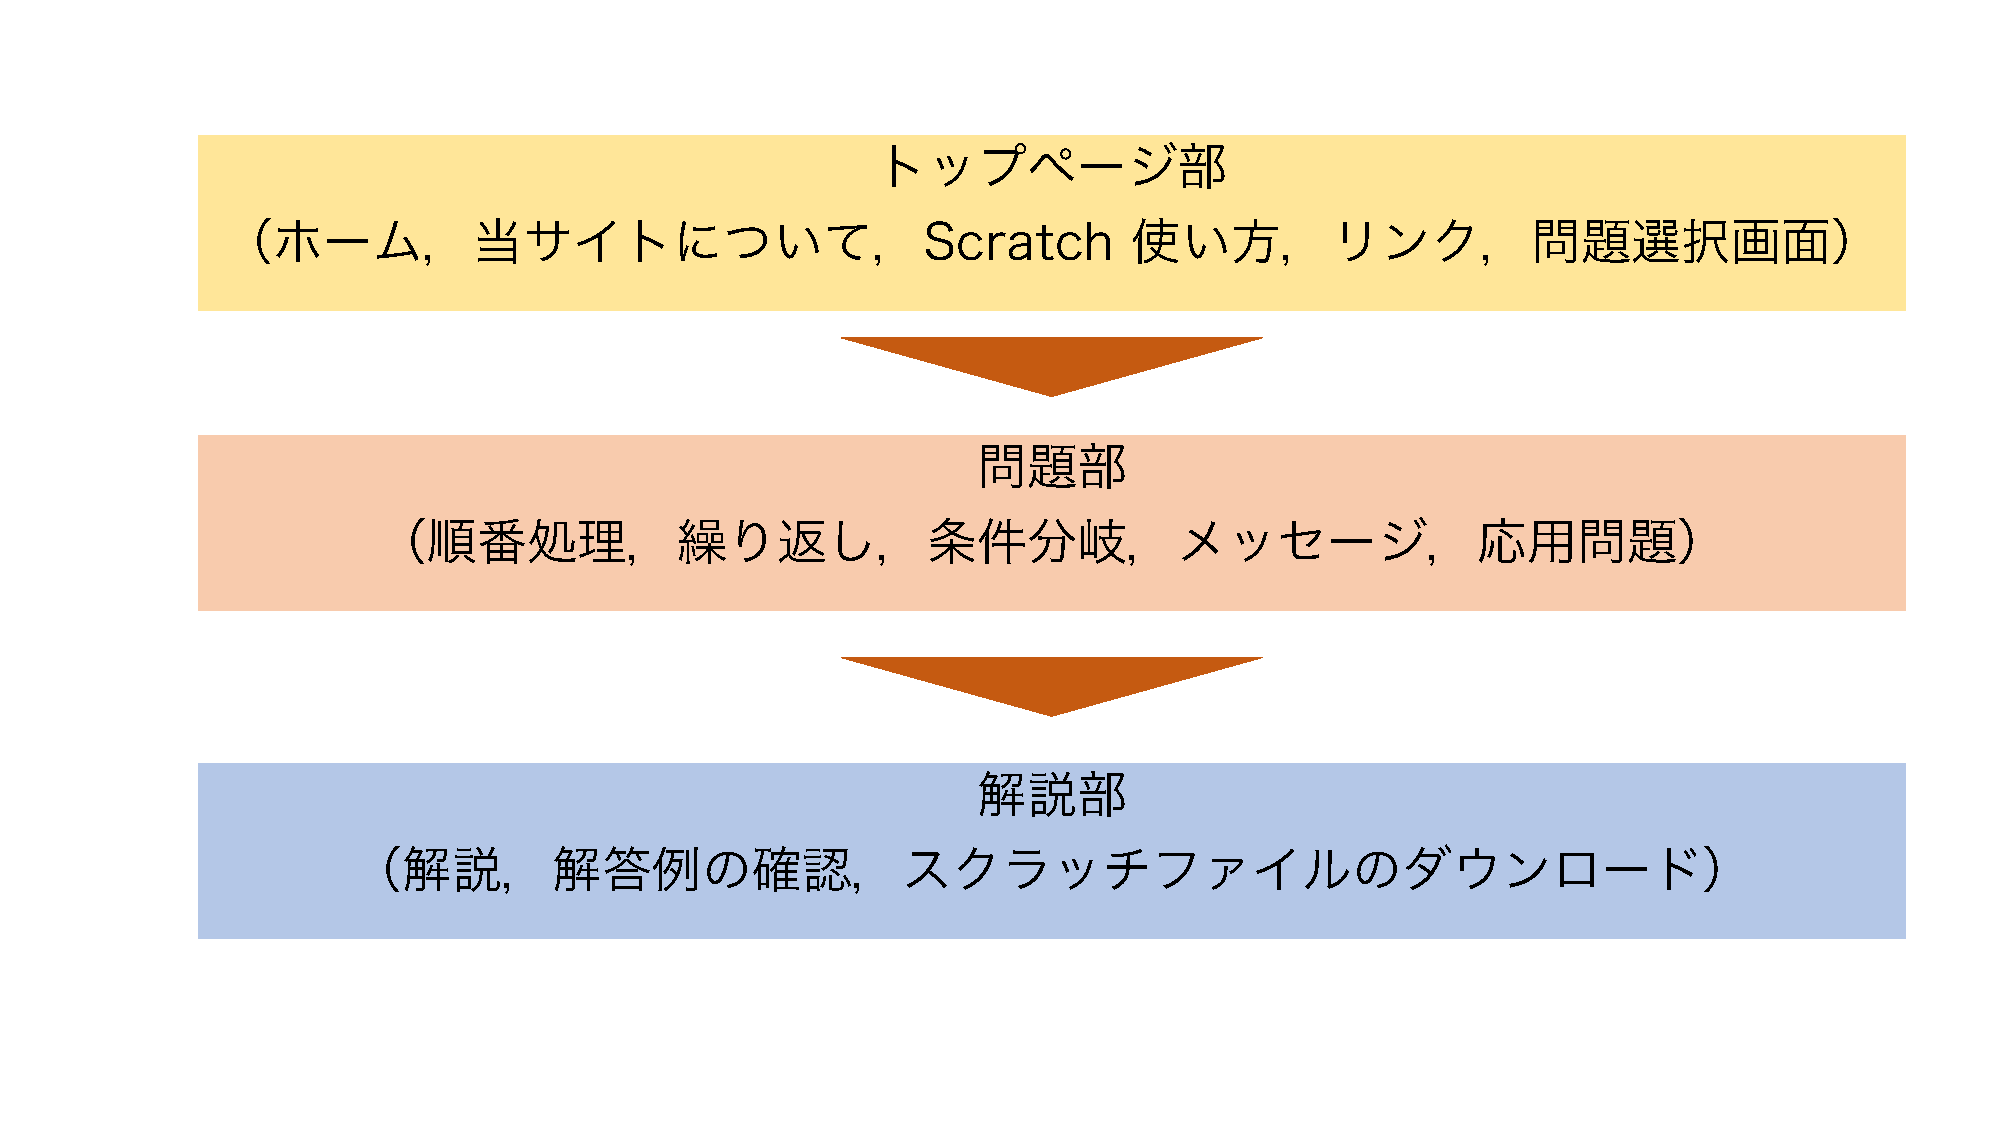
\includegraphics[width=15cm]{nagare.pdf}
\caption{サイト全体の流れ}
\label{fig:nagare}
\end{center}
\end{figure}
\newpage

\subsubsection{トップページ部}
課題集サイトのトップページ部分である.本サイトではホーム,当サイトについて,Scratch 使い方,問題選択画面,リンクから構成した.

\subsubsection{問題部}
サイト内で問題を出す部分である.問題は基本問題と応用問題から構成した.基本問題は「順番処理」,「繰り返し」,「条件分岐」,「メッセージ」の4つで構成した.

応用問題は基本問題を組み合わせて作成した発展的な問題である.

基本問題でのねらいを\ref{tab:nerai}に示す.
\begin{table}[htb]
\begin{center}
    \caption{トップページ部構成説明}
  \begin{tabular}{|c|c|} \hline
     処理名  & ねらい  \\ \hline
     順番処理& プログラムは上から下へ順に処理されていくこと \\ \hline
     繰り返し& 決まった回数や条件を満たすまで同じ処理を繰り返し行う \\ \hline
     条件分岐& 条件に応じて実行内容を切り替える \\ \hline
     メッセージ& 「〜を送る」と「〜を受け取ったとき」ブロックをセットで使いメッセージ処理を理解する \\ \hline
  \end{tabular}
  \label{tab:nerai}
  \end{center}
\end{table}
\subsubsection{解説部}
問題の解説部分である.問題の解答例,解説,スクラッチファイルのダウンロードを行うことができる.
\newpage

\subsection{基本問題部}
例として順番処理の問題を図\ref{fig:kihonrei}に示す.取り組んでもらう内容としては猫を10歩右に歩かせつつ大きさを50ずつ変えることである.
Scratchを用いてブロックを組み合わせ,課題を制作してもらうものとする.


\begin{figure}[h]
\begin{center}
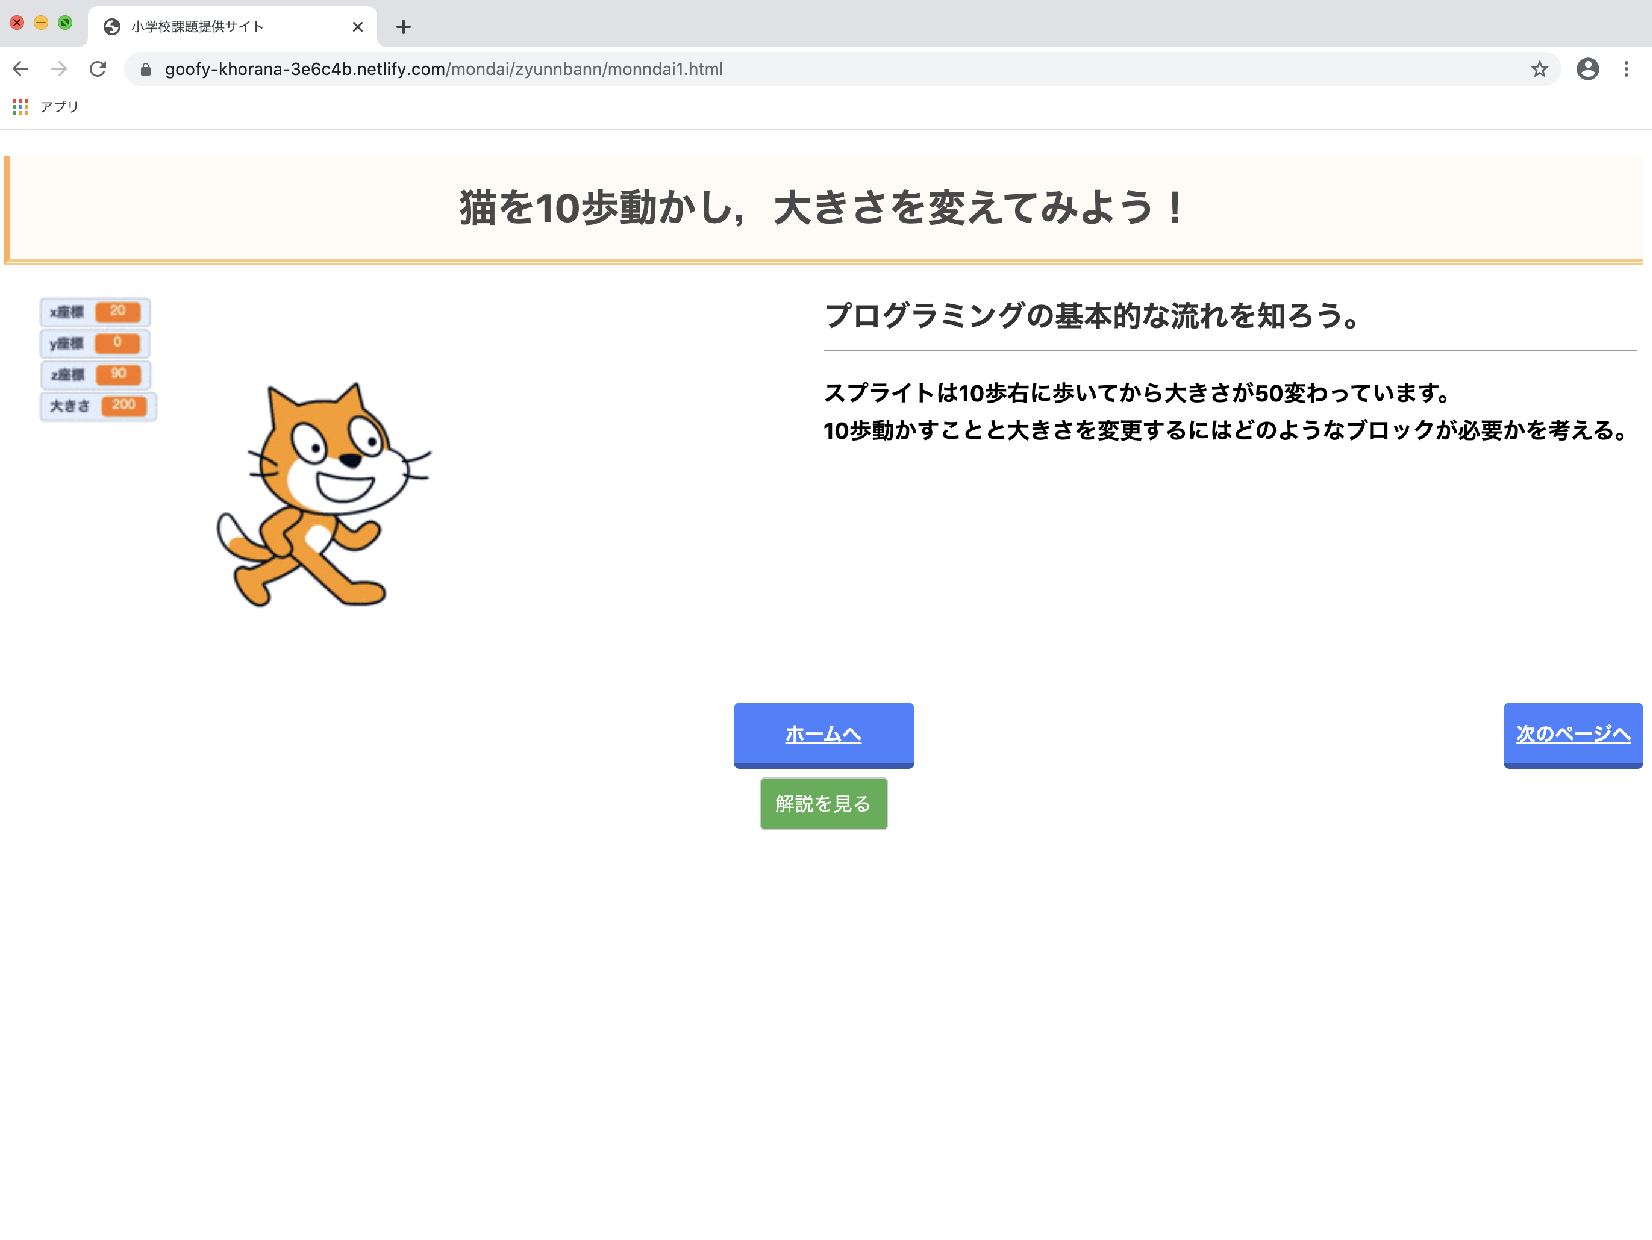
\includegraphics[width=15cm]{zyunnbanntoi.pdf}
\caption{基本問題 例}
\label{fig:kihonrei}
\end{center}
\end{figure}

\newpage

\subsubsection{基本問題部解説}
図\ref{fig:kihonreik}では「10歩動かす」命令と「大きさを50ずつ変える」の2つ命令を組み合わせることで,順番処理の基本である,上から下に処理していくことを学ぶことができる.

\begin{figure}[h]
\begin{center}
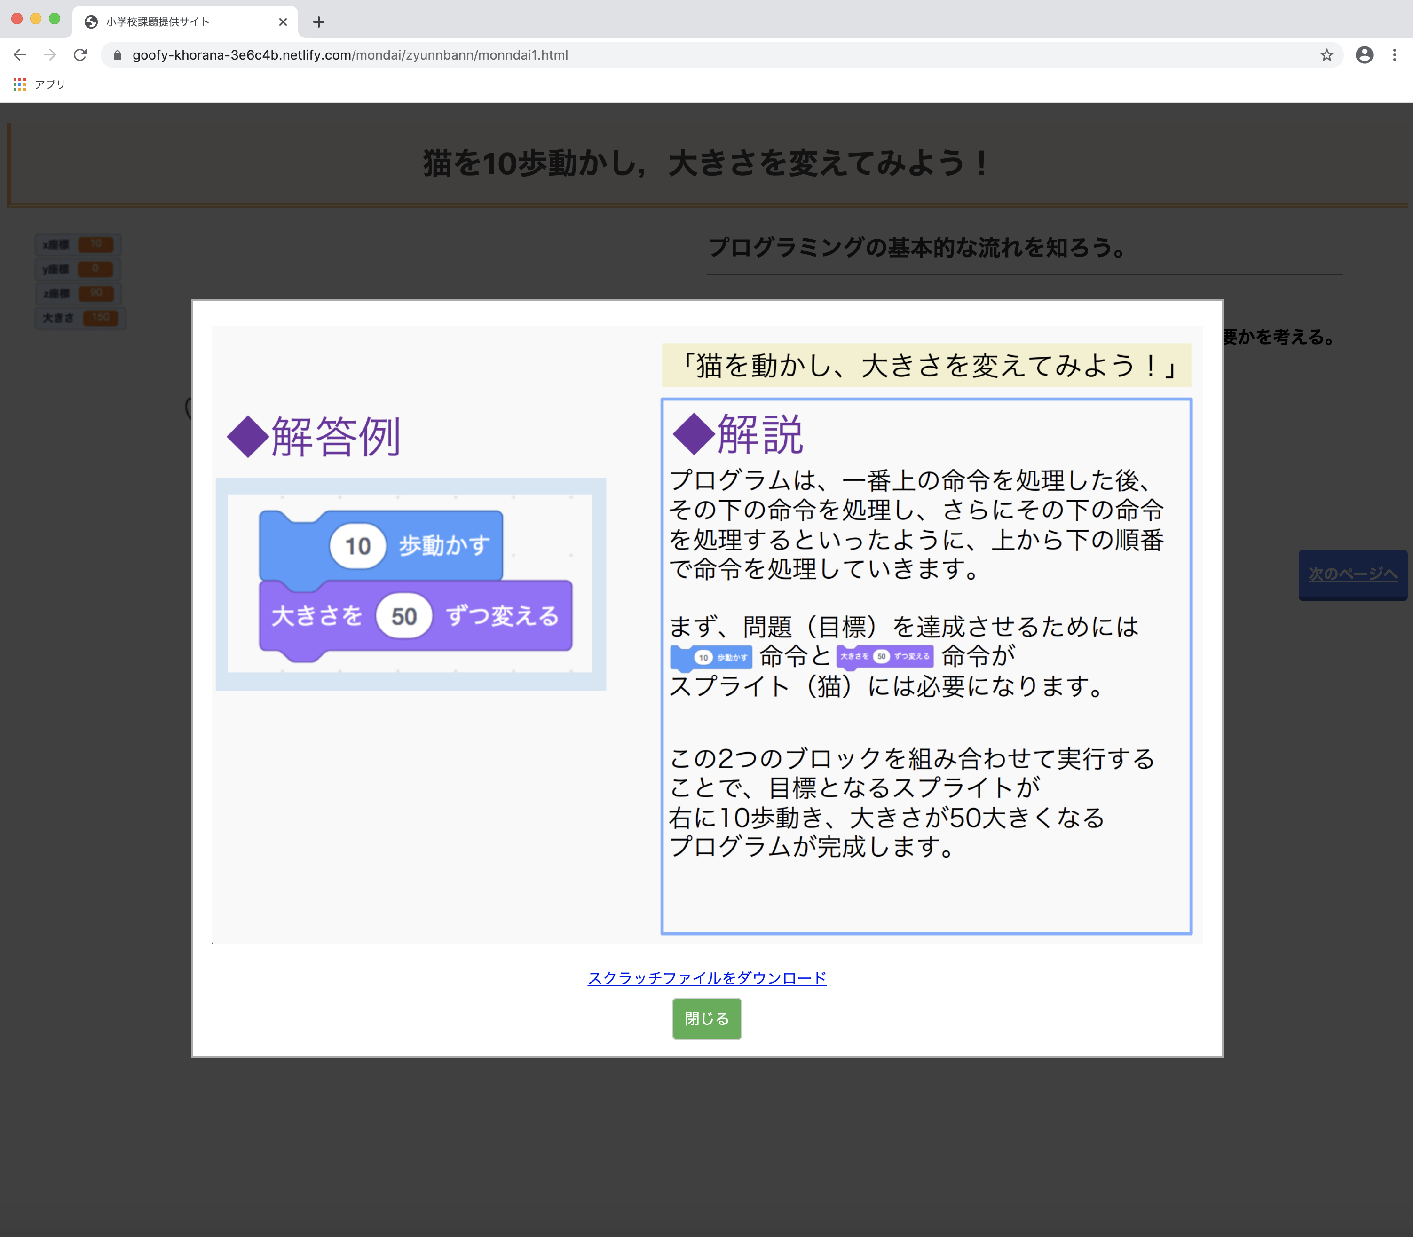
\includegraphics[width=15cm]{zyunnbannkotae.pdf}
\caption{基本問題部 解説 例}
\label{fig:kihonreik}
\end{center}
\end{figure}
\newpage

\subsection{応用問題部}
応用問題部の例として図\ref{fig:ouyou}に示す.
スプライトに問題を2つ問い,その答えをメッセージボックスに入力してもらう.
正解であれば「正解!」と2秒言い,不正解であれば「不正解!」と2秒言う.
2問答えた後に正解数に応じてスプライトが発言する内容が変わるプログラムである.



\begin{figure}[h]
\begin{center}
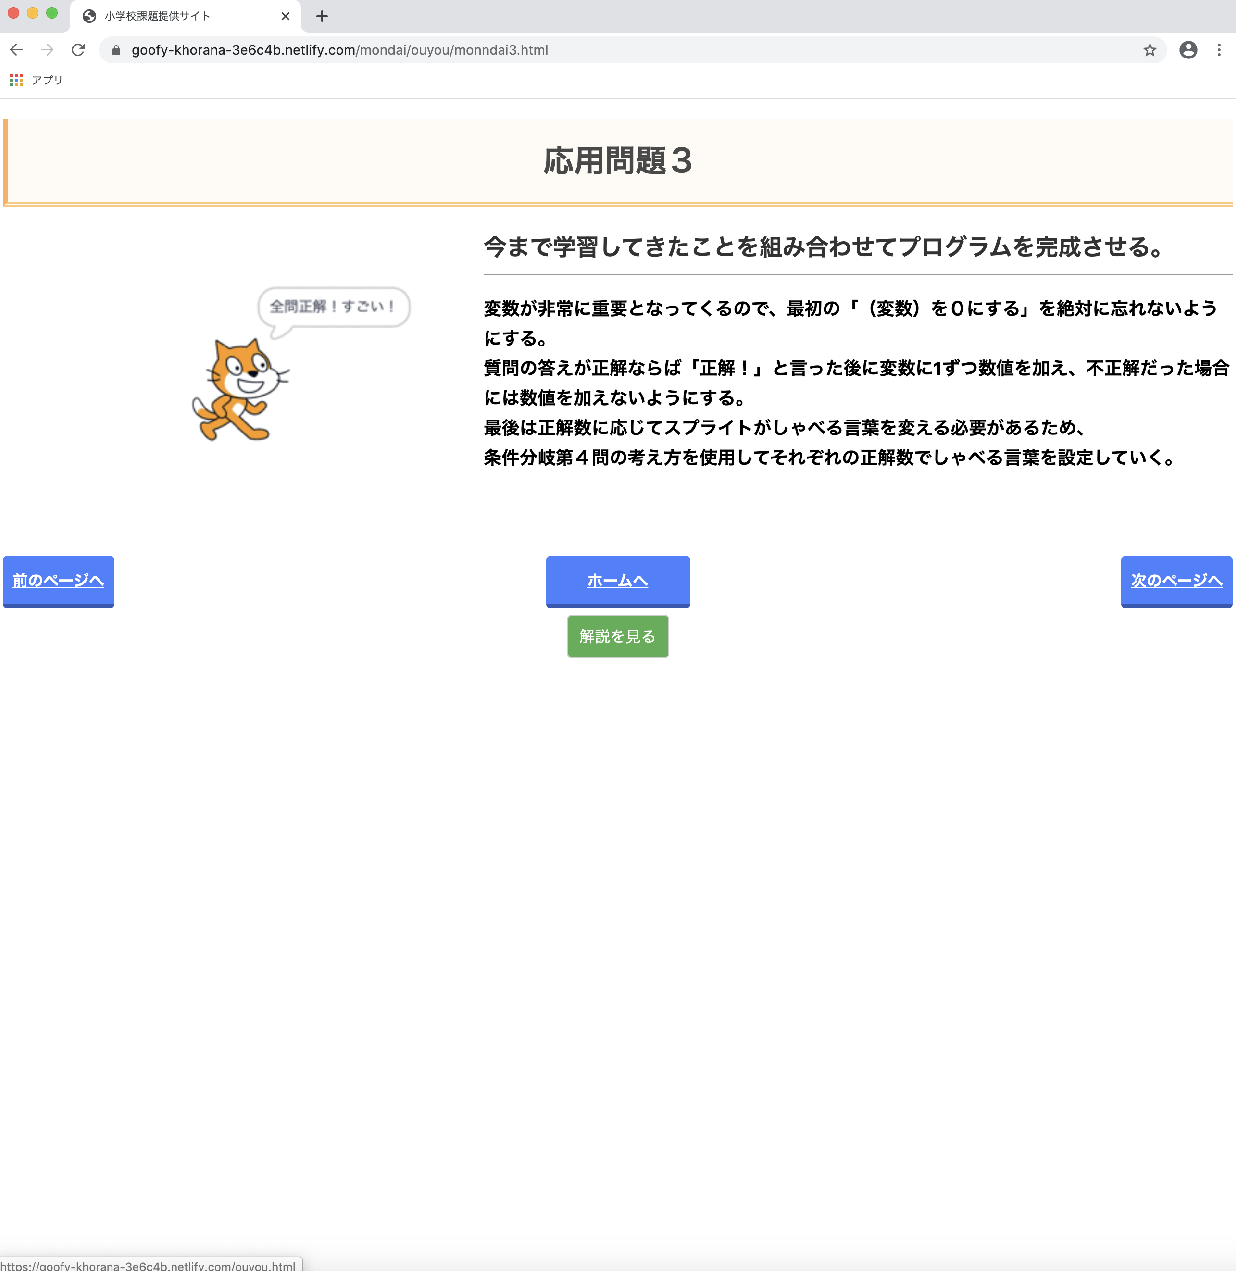
\includegraphics[width=15cm]{ouyoutoi.pdf}
\caption{応用問題部 例}
\label{fig:ouyou}
\end{center}
\end{figure}

\newpage

\subsubsection{応用問題部解説}
図\ref{fig:ouyouk}では正解数に応じてスプライトが発言する内容が変わることが重要である.そのため,スプライトが問題を正解した場合には変数を1変え,不正解の場合には変数を変えないといった処理が必要になる.




\begin{figure}[h]
\begin{center}
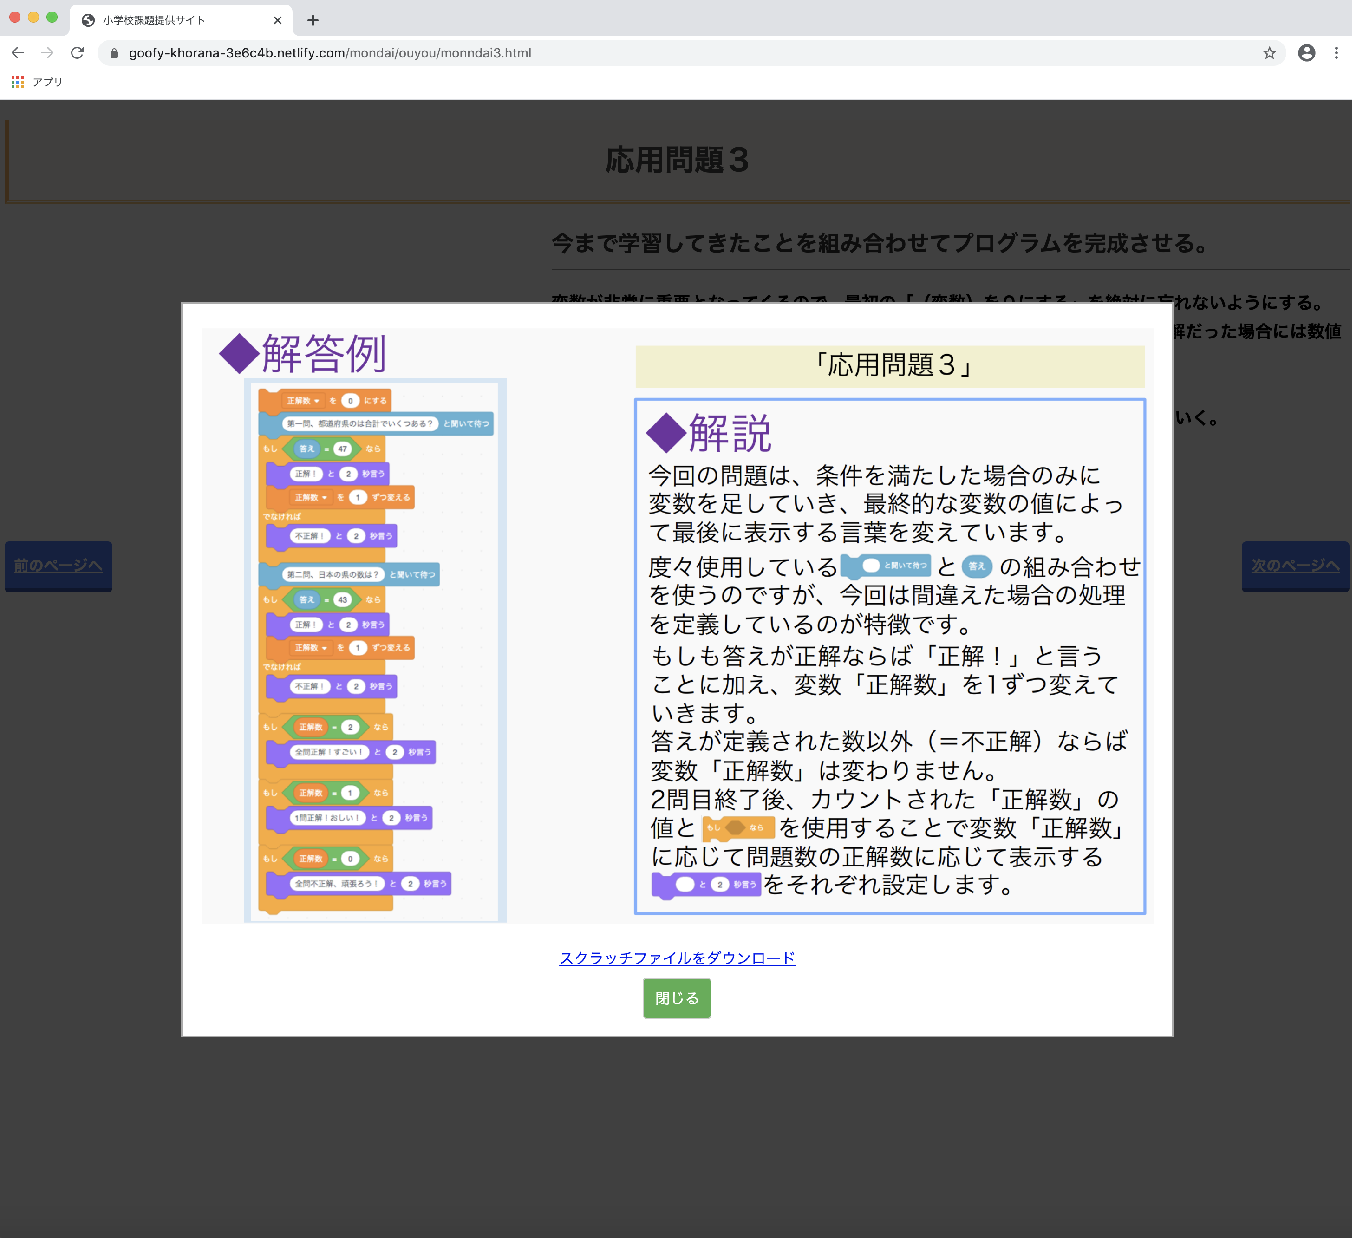
\includegraphics[width=15cm]{ouyoukotae.pdf}
\caption{応用問題部 解説 例}
\label{fig:ouyouk}
\end{center}
\end{figure}




%!TEX root = 0卒業論文.tex
\clearpage

\section{\rm 教材の使用方法}

\subsection{学習方法}
学習方法の流れを図\ref{fig:gakunagare}に示す.授業で教員や児童がパソコン又はiPadを用いて本サイトを使用してもらうことを想定する.
本サイトの,トップページ部,Scratch 使い方の画面を参照し,Scratchの基本動作を学んでもらう.
授業内では問題画面を児童に見ていただき,問題画面,表示される制作課題のアニメーションと同じ動きになるものをScratchを用いて作成する.
作成した後に,「解説を見る」ボタンを押し,解答例,解説を読み理解してもらう流れになる.
また,スクラッチファイルをダウンロードすることが可能になため,自身で動作を確認することができる.
\begin{figure}[h]
\begin{center}
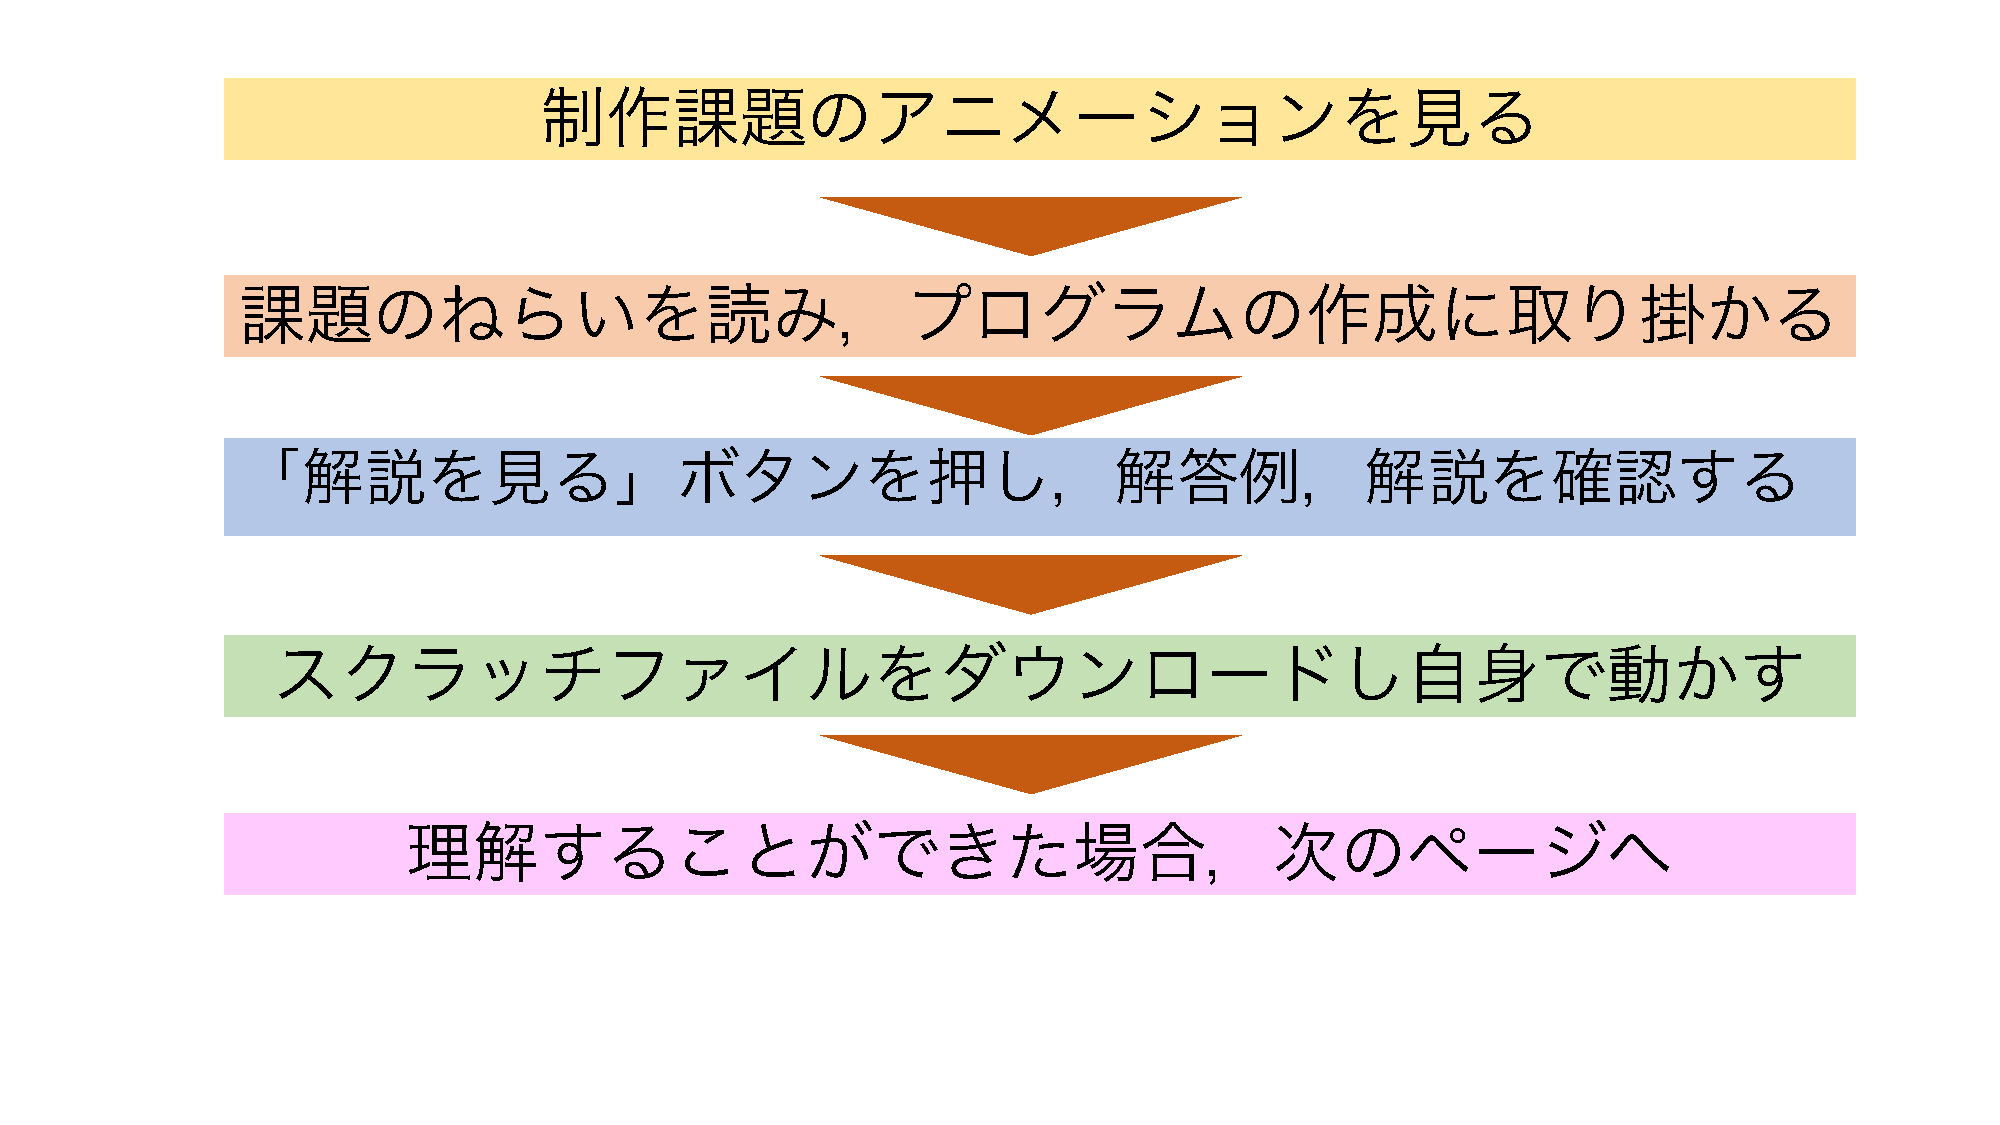
\includegraphics[width=15cm]{gakushuu.pdf}
\caption{学習方法 流れ}
\label{fig:gakunagare}
\end{center}
\end{figure}


%!TEX root = 0卒業論文.tex
\newpage

\section{\rm サイトの説明}
\subsection{画面説明}
制作したサイトでは主にトップページ画面,問題画面,解説画面の3つの画面が存在する.

\subsubsection{トップページ画面}
図\ref{fig:topgamen1}は,本サイトのトップページである.サイトを開いた時,最初に開かれるページである.

\begin{figure}[h]
\begin{center}
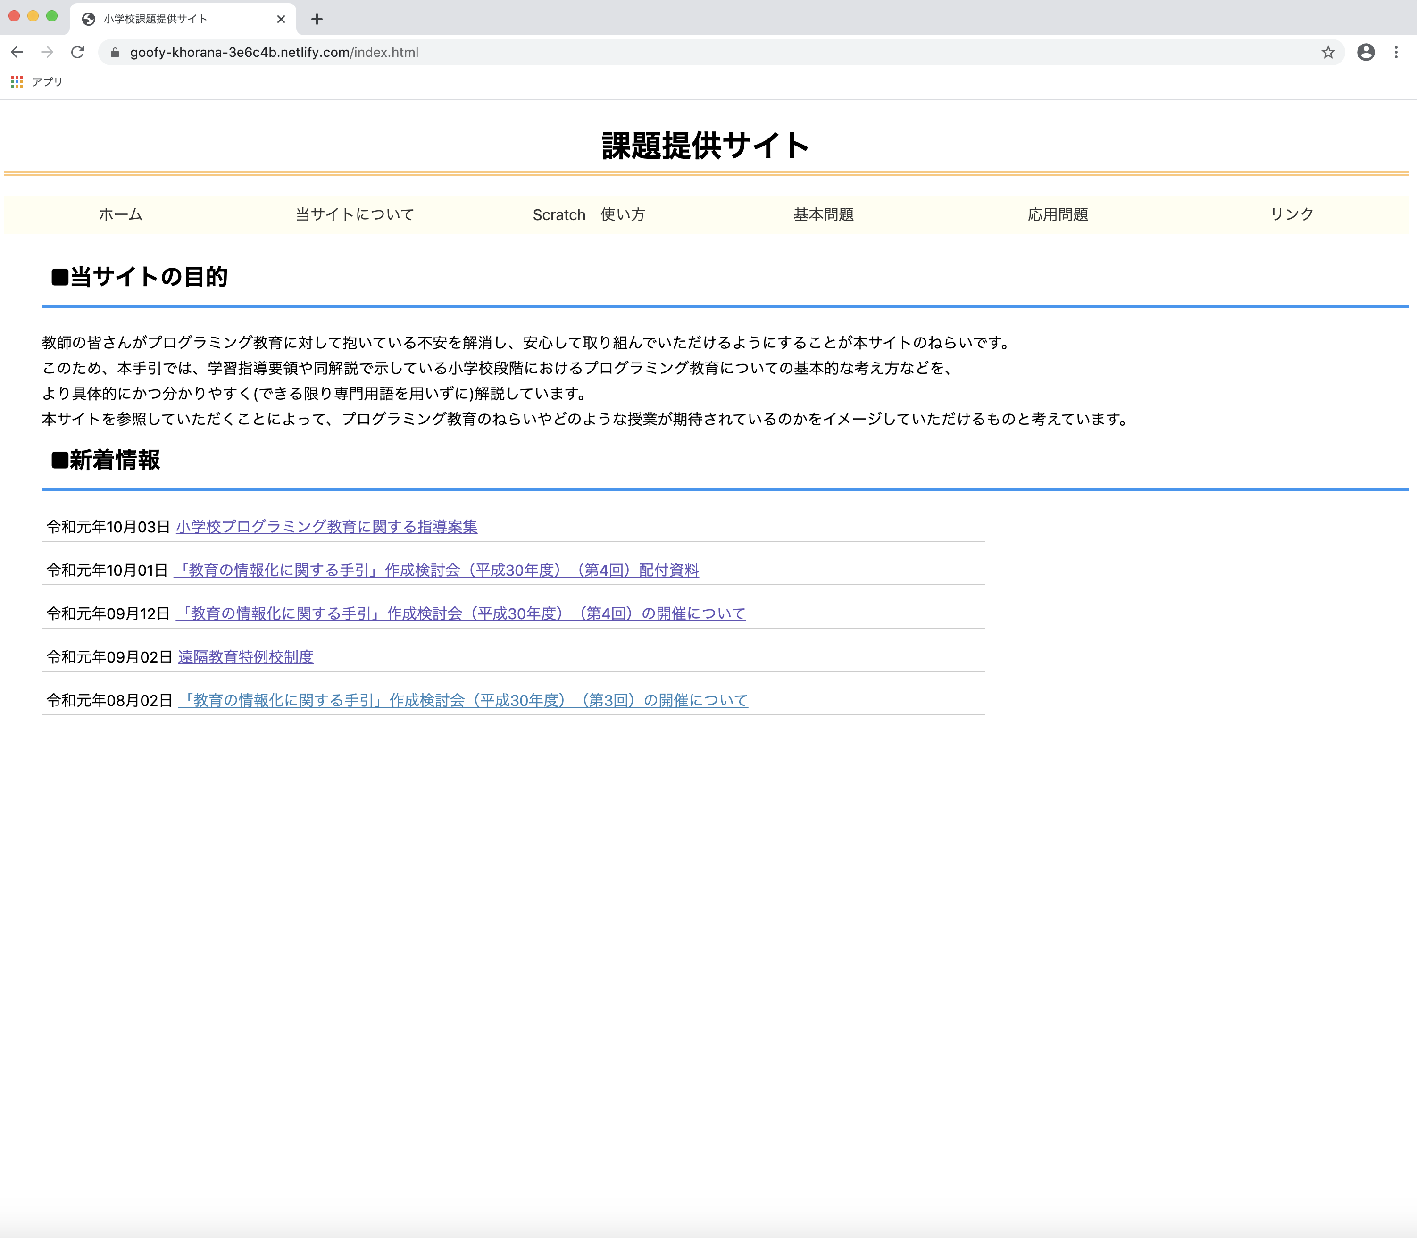
\includegraphics[width=15cm]{toppage.pdf}
\caption{トップページ画面}
\label{fig:topgamen1}
\end{center}
\end{figure}

\newpage
\subsubsection{サイト使用方法画面}
図\ref{fig:tougamen}は,「当サイトについて」である.ここではサイト利用上での注意点を示している.
\begin{figure}[h]
\begin{center}
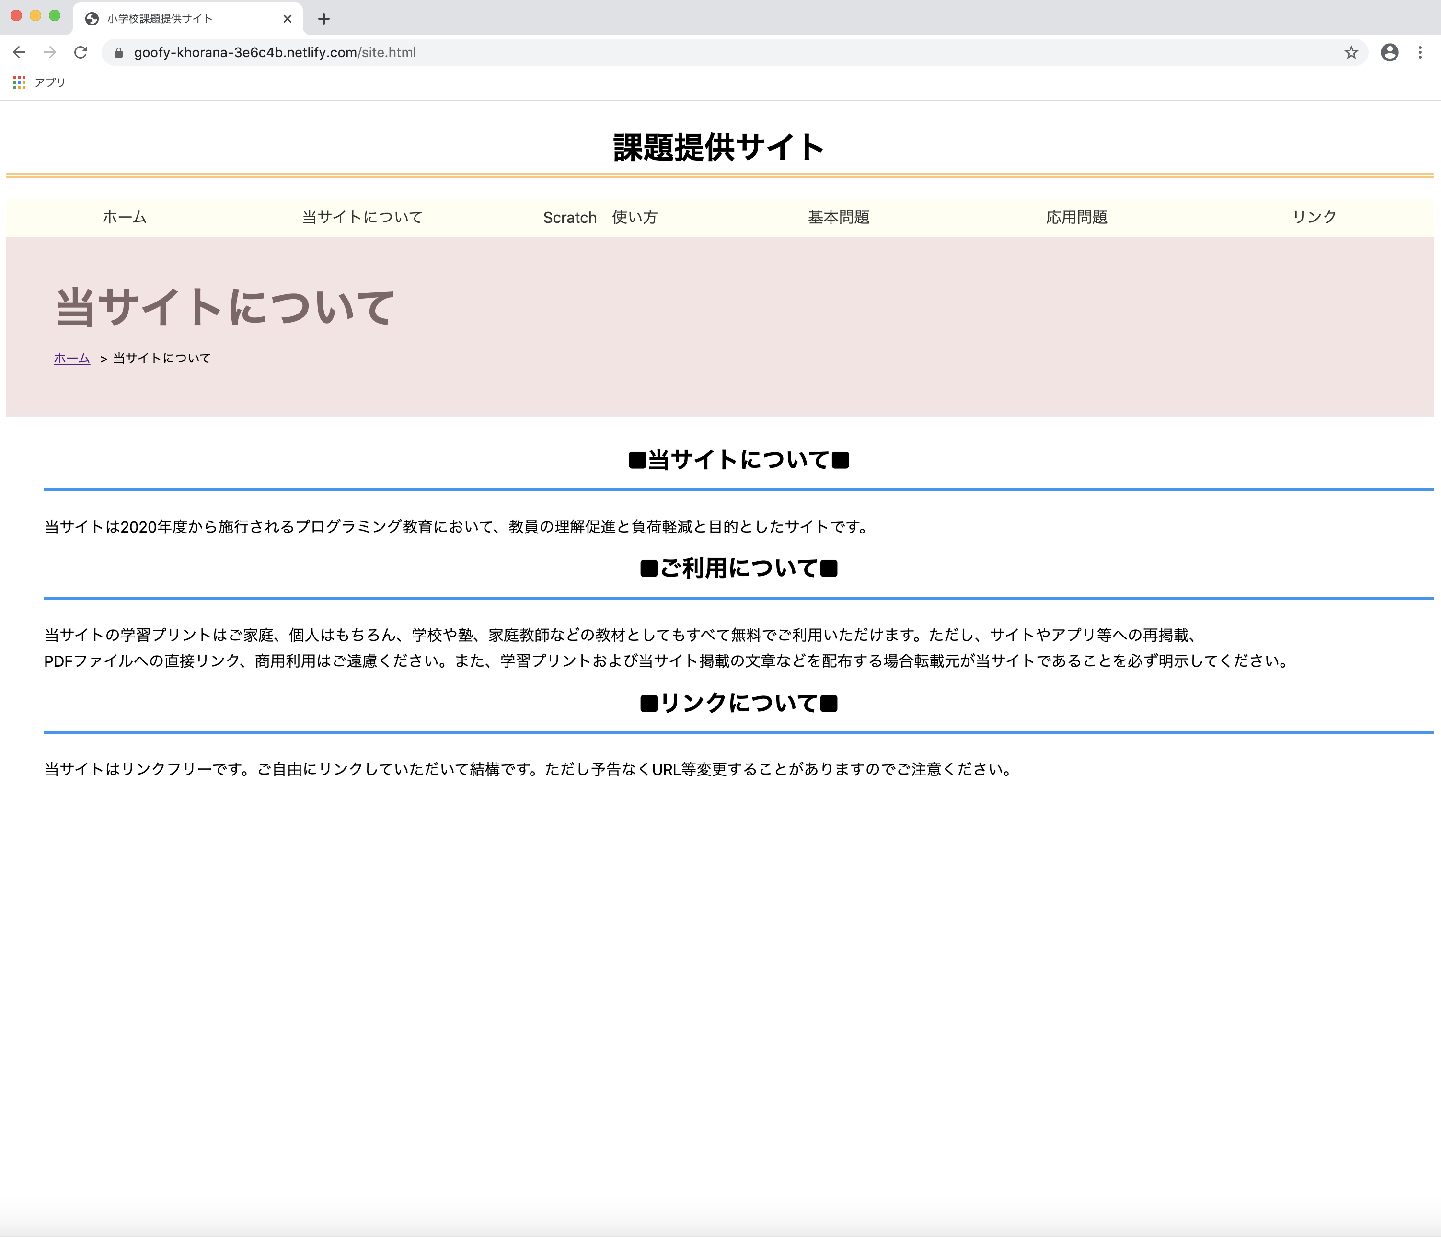
\includegraphics[width=15cm]{site.pdf}
\caption{当サイトについて画面}
\label{fig:tougamen}
\end{center}
\end{figure}

\newpage

\subsubsection{Scrartch使用方法画面}
図\ref{fig:tukaigamen}は,「Scratch使用方法」である.この画面では実際にScratchを使用したことがない方のために,Scratchの使用方法を簡単に説明した画面である.

\begin{figure}[h]
\begin{center}
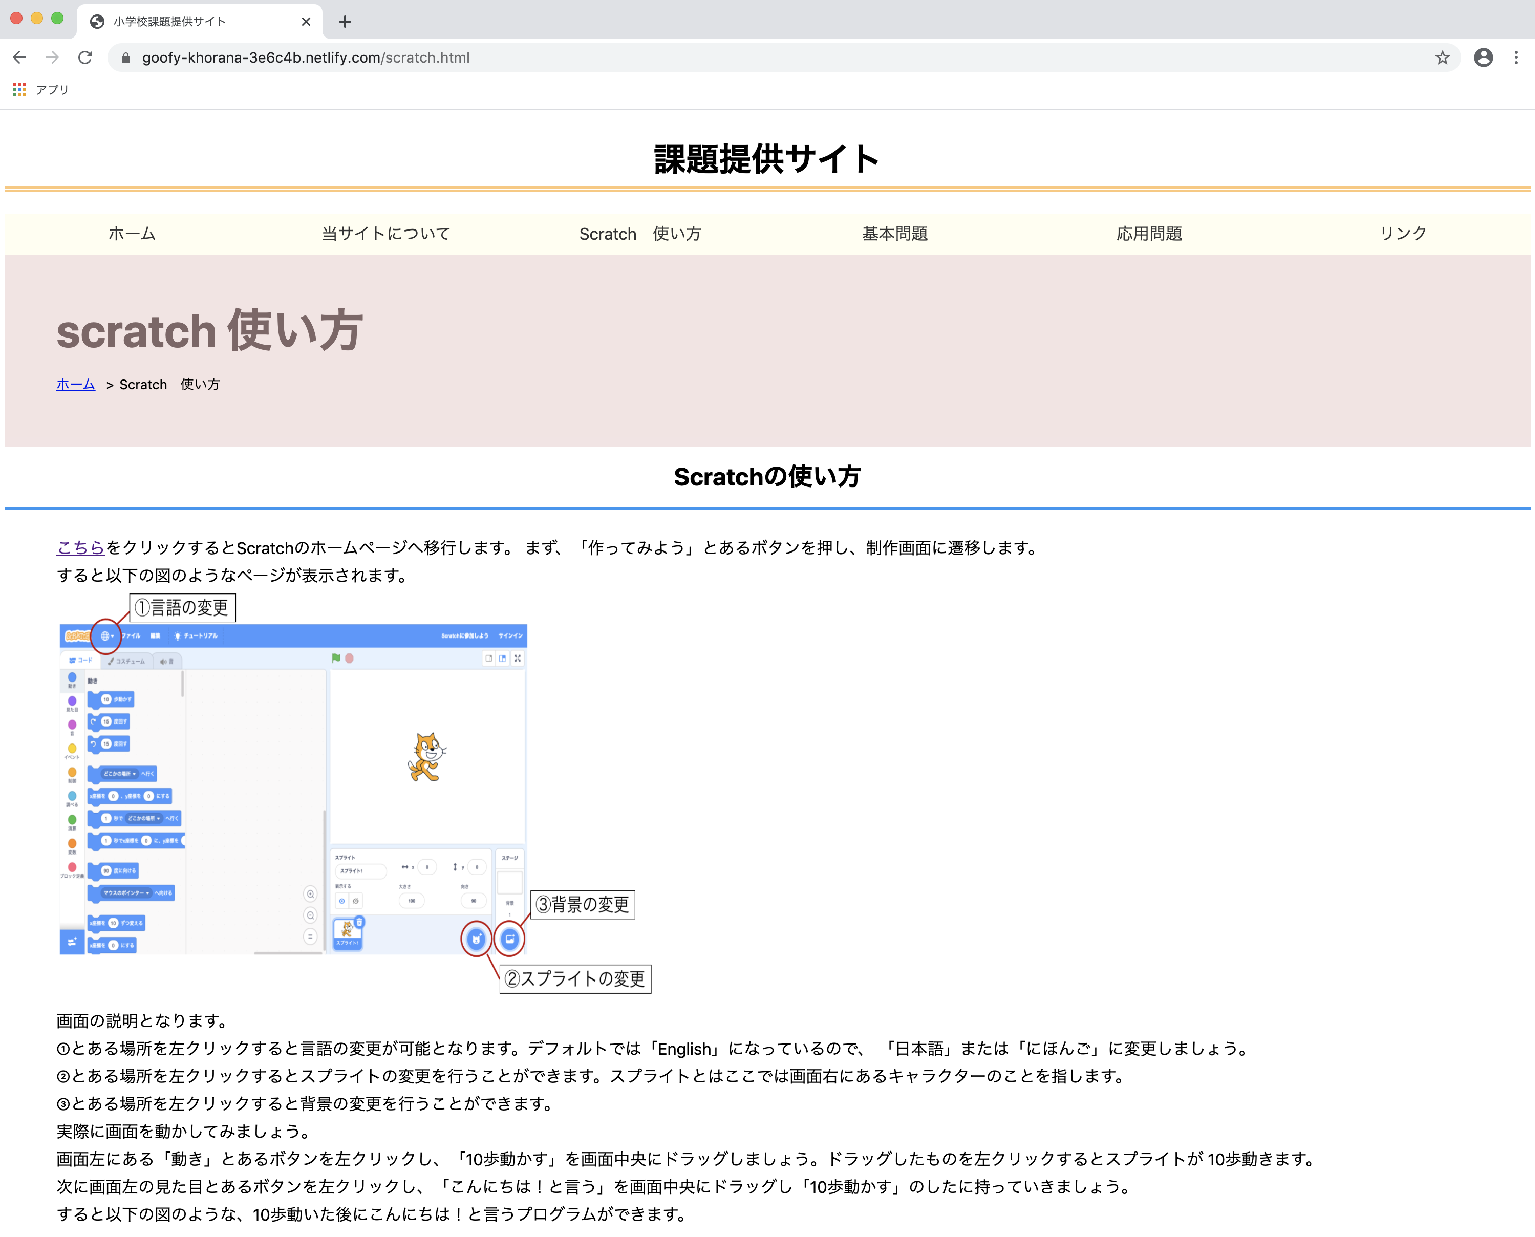
\includegraphics[width=15cm]{Scratch.pdf}
\caption{Scratch 使い方画面}
\label{fig:tukaigamen}
\end{center}
\end{figure}

\newpage

\subsubsection{リンク画面}
図\ref{fig:linkgamen}は,様々なリンクが表示される.文部科学省や学習指導要領など授業で役立つリンクを配置した.

\begin{figure}[h]
\begin{center}
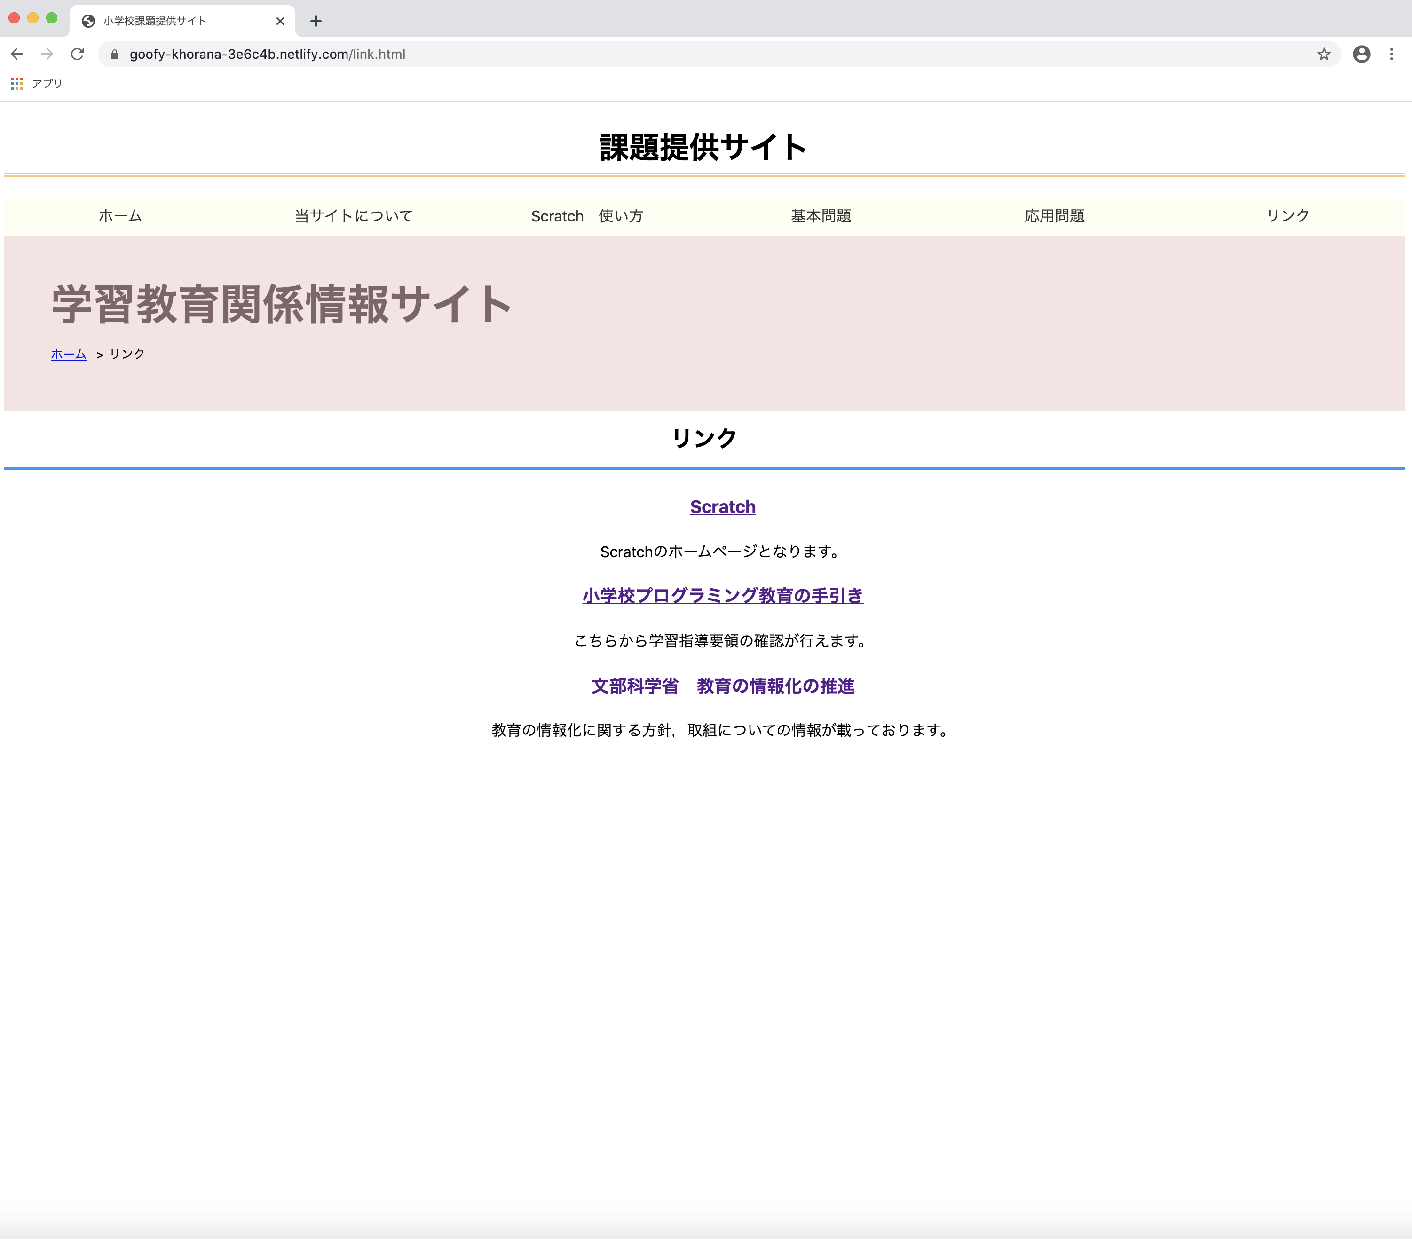
\includegraphics[width=15cm]{Link.pdf}
\caption{リンク画面}
\label{fig:linkgamen}
\end{center}
\end{figure}

\newpage

\subsubsection{問題選択画面}
図\ref{fig:mondaisentaku}は,問題を選択する画面である.ここでは例として順番処理のページを示す.

\begin{figure}[h]
\begin{center}
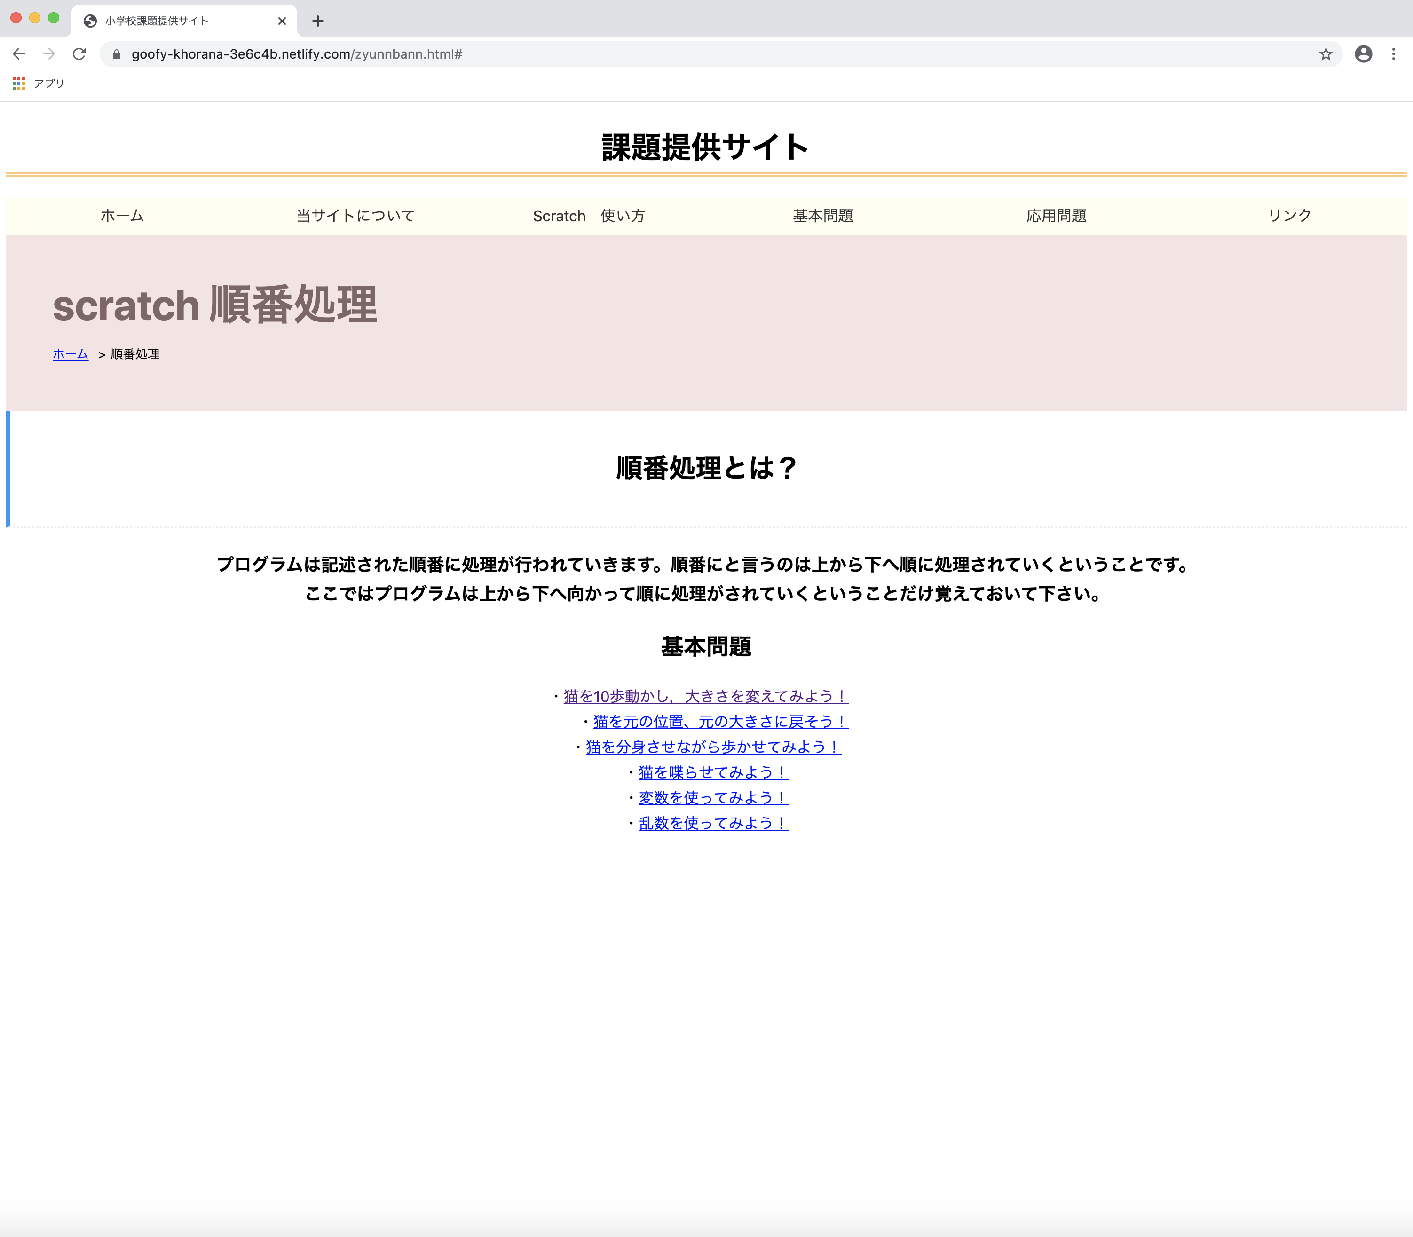
\includegraphics[width=15cm]{zyunnbann.pdf}
\caption{問題選択画面}
\label{fig:mondaisentaku}
\end{center}
\end{figure}

\newpage

\subsection{問題画面}

図\ref{fig:mondaigamen1}は,サイトの問題部分で表示される.この画面で問題が出題される.画面はタイトル部,アニメーション部,ねらい部,ボタン部に分かれている.
各部の説明を表\ref{tab:site1}に示す.
\begin{table}[htb]
\begin{center}
    \caption{問題部画面構成要素説明}
  \begin{tabular}{|c|c|} \hline
     要素名  & 説明  \\ \hline
     タイトル部& 課題のタイトルを部分 \\ \hline
      アニメーション部& 達成すべき目標となるアニメーションを表示する部分 \\ \hline
      ねらい部& 課題を取り組む上でのねらいを表示する部分 \\ \hline
      ボタン部& ホームに戻る,次のページへ,問題の解説を表示する部分\\ \hline
  \end{tabular}
  \label{tab:site1}
  \end{center}
\end{table}
\begin{figure}[h]
\begin{center}
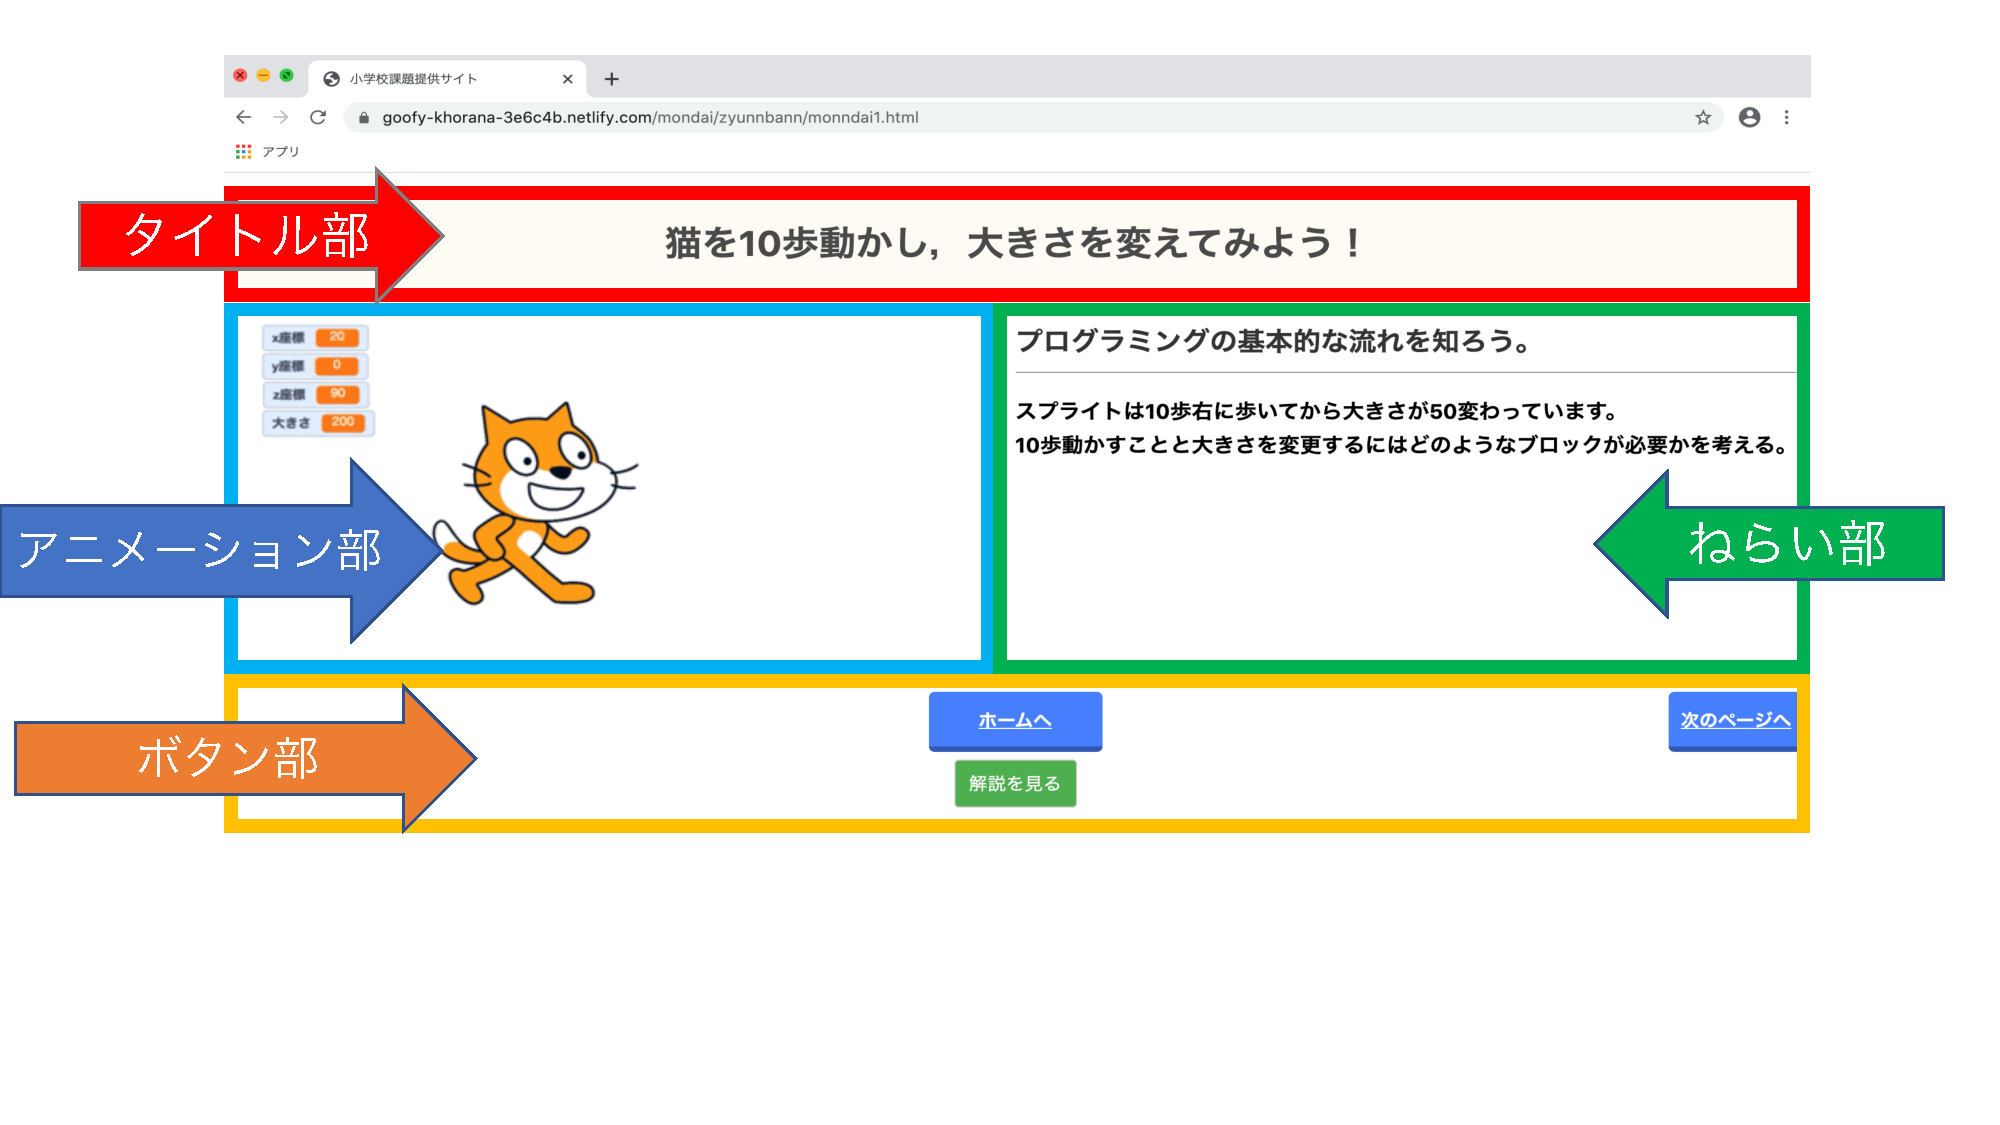
\includegraphics[width=15cm]{mondaigamen.pdf}
\caption{問題画面}
\label{fig:mondaigamen1}
\end{center}
\end{figure}

\newpage

\subsection{解説画面}
図\ref{fig:zyunnbannkaisetu}は,問題画面の「解説を見る」ボタンを押すことで表示される.
\begin{figure}[h]
\begin{center}
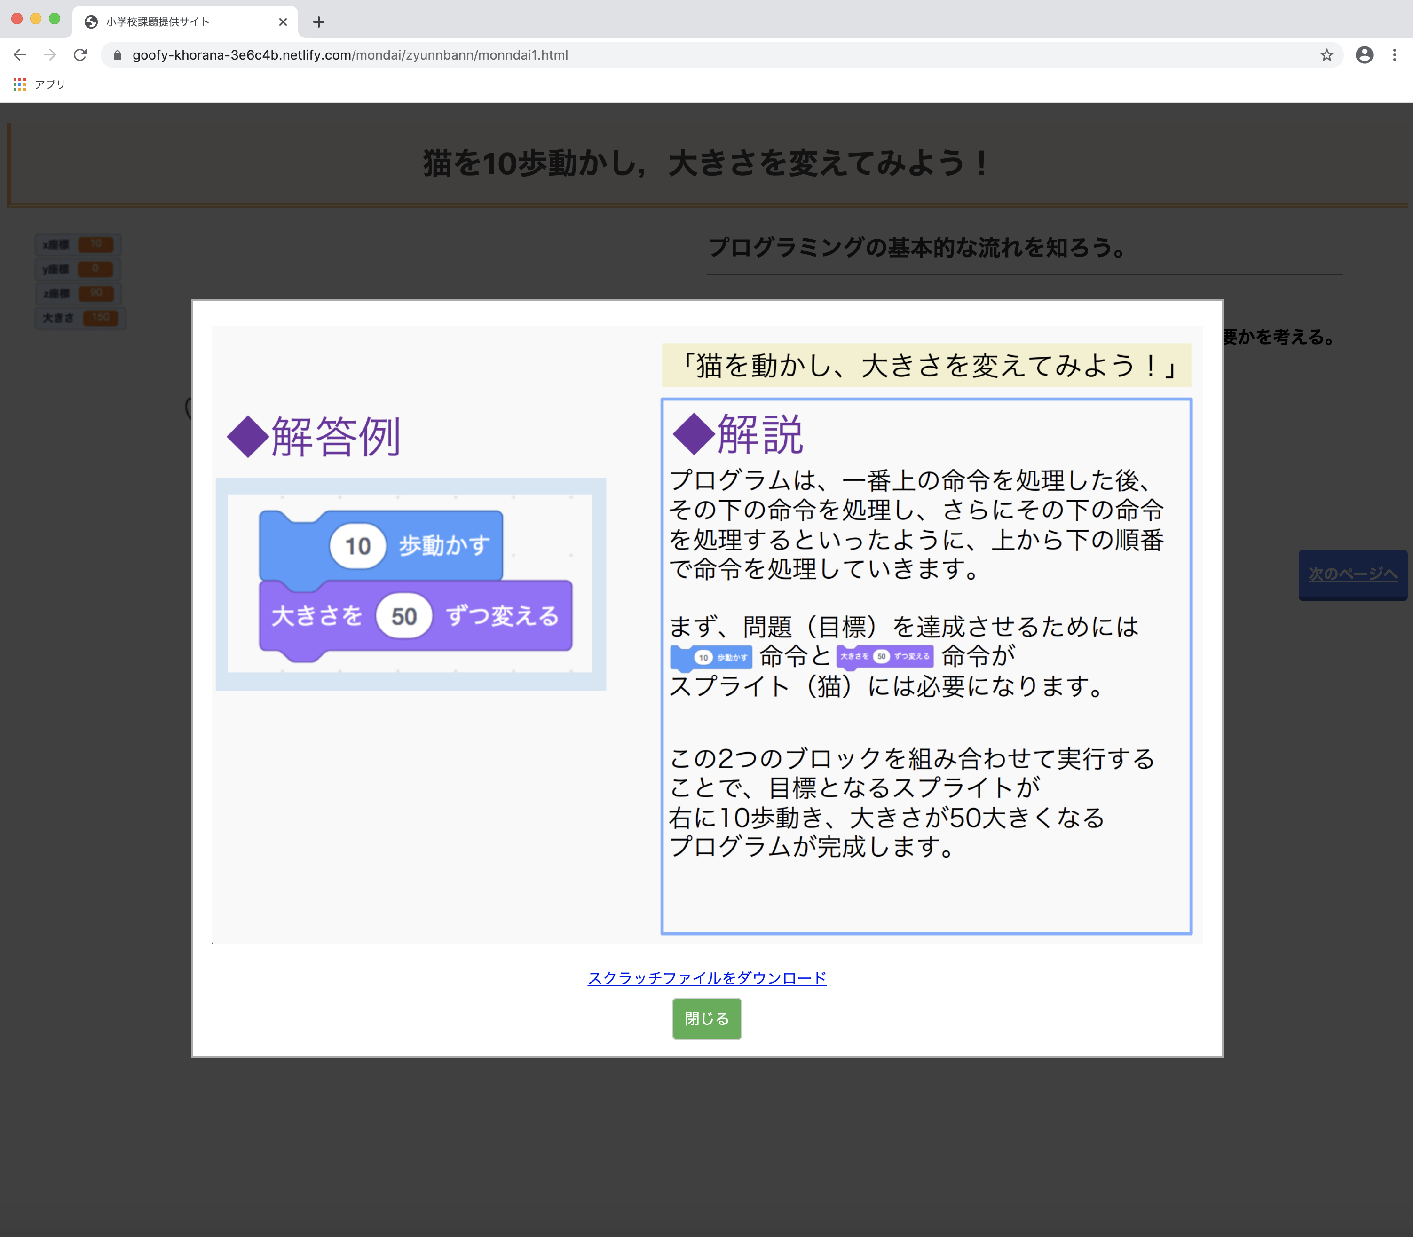
\includegraphics[width=15cm]{zyunnbannkotae.pdf}
\caption{解説画面}
\label{fig:zyunnbannkaisetu}
\end{center}
\end{figure}

\newpage


\subsection{操作説明}
サイトの操作説明を行う.トップページ画面,問題画面,解説画面はページ遷移ボタンのみである.
\subsubsection{問題画面の流れ}
\begin{enumerate}
 \item 課題のテーマが問題画面上部に表示される
 \item 出された課題を達成するため,課題のアニメーション,課題のねらいを読み,取り組む.
 \item 「解説を見る」を押し,解説とスクラッチファイルを用いて課題を理解する.
 \item 理解できたのであれば,「次のページへ」ボタンで画面遷移する. 
\end{enumerate}



















%!TEX root = 0卒業論文.tex
\clearpage

\section{\rm 教材の設計}

\subsection{トップページ部}
トップページ部では9つのファイルで構成したサイトのトップページ部分である.
各ファイルの説明を表\ref{tab:topsetumei}に示す.
\begin{table}[htb]
\begin{center}
    \caption{トップページ部構成説明}
  \begin{tabular}{|c|c|} \hline
     ファイル名  & 説明  \\ \hline
     home.html& サイトのトップページとなる部分 \\ \hline
     site.html& サイトの利用方法や注意点を示す \\ \hline
     zyunnbann.html& 順番処理の問題選択画面 \\ \hline
     kurikaesi.html& 繰り返しの問題選択画面 \\ \hline
     zyoukennbunnki.html& 条件分岐の問題選択画面 \\ \hline
     message.html& メッセージの問題選択画面 \\ \hline
     ouyou.html& 応用問題の問題選択画面 \\ \hline
     scratch.html& Scratchの使用方法に関する部分 \\ \hline
     link.html& Scratch,文部科学省,学習指導要領のリンク\\ \hline
  \end{tabular}
  \label{tab:topsetumei}
  \end{center}
\end{table}
\newpage

\subsection{問題部}
問題部では制作した問題を出題する.

\subsubsection{順番処理}
順番処理の問題構成を表\ref{tab:zyunnbannhyou}に示す.
\begin{table}[htb]
\begin{center}
    \caption{順番処理構成説明}
  \begin{tabular}{|c|c|} \hline
     ファイル名  & 問題タイトル  \\ \hline
     monndai1.html& 猫を10歩動かし,大きさを変えてみよう! \\ \hline
     monndai2.html& 猫を元の位置、元の大きさに戻そう! \\ \hline
     monndai3.html& 猫を分身させながら歩かせてみよう! \\ \hline
     monndai4.html& 猫を喋らせてみよう! \\ \hline
     monndai5.html& 変数を使ってみよう! \\ \hline
     monndai6.html& 乱数を使ってみよう! \\ \hline
  \end{tabular}
  \label{tab:zyunnbannhyou}
  \end{center}
\end{table}

\subsubsection{繰り返し}
繰り返しの構成を表\ref{tab:kurikaesihyou}に示す.

\begin{table}[htb]
\begin{center}
    \caption{繰り返し構成説明}
  \begin{tabular}{|c|c|} \hline
     ファイル名  & 問題タイトル  \\ \hline
     monndai1.html& ループを使ってみよう! \\ \hline
     monndai2.html& 猫を鳴かせてみよう! \\ \hline
     monndai3.html& 猫をずっと歩かせてみよう! \\ \hline
     monndai4.html& 背景を変え続けてみよう! \\ \hline
     monndai5.html& 猫にアニメーションをつけてみよう! \\ \hline
     monndai6.html& 回数を指定したループを使ってみよう! \\ \hline
     monndai7.html& 時間を指定したループを使ってみよう! \\ \hline
     monndai8.html& 様々な条件をループに組み込もう! \\ \hline
     monndai9.html& ループの中にループを組み込んでみよう!1 \\ \hline
     monndai10.html& ループの中にループを組み込んでみよう!2 \\ \hline
     monndai11.html& ループの中にループを組み込んでみよう!3 \\ \hline
  \end{tabular}
  \label{tab:kurikaesihyou}
  \end{center}
\end{table}
\newpage

\subsubsection{条件分岐}
条件分岐処理の構成を表\ref{tab:zyoukenhyou}に示す.

\begin{table}[htb]
\begin{center}
    \caption{条件分岐構成説明}
  \begin{tabular}{|c|c|} \hline
     ファイル名  & 問題タイトル  \\ \hline
     monndai1.html& 足し算の答えを確認してみよう! \\ \hline
     monndai2.html& 特定の座標でのみ処理を行わせよう! \\ \hline
     monndai3.html& キーやマウスを条件に設定してみよう \\ \hline
     monndai4.html& 2つの条件下で動くプログラムを作ろう \\ \hline
     monndai5.html& 条件を満たしたときにループさせよう \\ \hline
     monndai6.html& 条件をさらに詳しく定義しよう \\ \hline
     monndai7.html& ループ中に条件分岐をさせてみよう \\ \hline
     monndai8.html& 1つのブロック2つの処理を用意する1 \\ \hline
     monndai9.html& 1つのブロック2つの処理を用意する2\\ \hline
  \end{tabular}
  \label{tab:zyoukenhyou}
  \end{center}
\end{table}

\subsubsection{応用問題}
応用問題の構成を表\ref{tab:ouyouhyou}
\begin{table}[htb]
\begin{center}
    \caption{応用問題構成説明}
  \begin{tabular}{|c|c|} \hline
     ファイル名  & 問題のねらい  \\ \hline
     monndai1.html& 今まで学習してきたことを組み合わせてプログラムを完成させる \\ \hline
     monndai2.html& 今まで学習してきたことを組み合わせてプログラムを完成させる \\ \hline
     monndai3.html& 今まで学習してきたことを組み合わせてプログラムを完成させる \\ \hline
     monndai4.html& 今まで学習してきたことを組み合わせて自分自身で創作物を完成させる \\ \hline
  \end{tabular}
  \label{tab:ouyouhyou}
  \end{center}
\end{table}


\subsection{解説部}
問題部下部に示す,「解説を見る」ボタンを押すことでモーダルウィンドウが開く.ウィンドウ内にて各問題ごとのスクラッチファイルのダウンロード,解答例,解説を表示する.














%!TEX root = 0卒業論文.tex
\newpage

\section{\rm 結言}

近年の情報化社会への急激な移り変わりや,IT技術者不足の背景などを受け,文部科学省が2020年以降に従来の教育にプログラミング教育を盛り込んだ学習指導要領改定案を発表した.
これにより小学校低学年時からプログラミング教育が実施されることになり,児童のプログラミング教育に注目が集まっている.

しかし,2020年に向けてプログラミングの授業に関する研修は各々行われているものの,授業を行えるか不安と感じる教職員が多い.


さらに,ビジュアルプログラミングの解説と例題の提供を同時に行なっているビジュアルプログラミング教材が不足しており,
ビジュアルプログラミングを学習した後,教職員は自分で授業用の例題を作成するか,別の教材や問題集などから授業で扱う例題などを引用してくる必要がある.


本研究では, 小学校プログラミング教育への導入, プログラミング的思考力を身につける, 教職員のプログラミング教育への知識不足による不安と負担を解消することのできるWebサイトを用いたプログラミング教材を制作した.

「Scratch」を用いて, 文部科学省が提唱した「プログラミング的思考」を構成する「自らの意図を明確化させる思考力」「どのような動きをどのような順序でさせれば良いのかを考える思考力」「どのように組み合わせれば良いかを考える思考力」を育成することを目的とした.


%!TEX root = 0卒業論文.tex
\newpage
\section*{謝辞}
\addcontentsline{toc}{section}{謝辞}

本研究の遂行及び本論文の作成にあたり,須田研究室の仲間と実験にご協力いただいた皆様に深く感謝の意を表します.

そして,何よりも本論文の作成にあたり,多大なる御指導及び御助言を頂きました須田 宇宙准教授に深く感謝の意を表します.


%!TEX root = 0卒業論文.tex
\newpage

\addcontentsline{toc}{section}{参考文献}

\begin{thebibliography}{5}

\bibitem{yuushiki} 「小学校段階における論理的思考力や創造性、問題解決能力等の育成とプログラミング教育に関する有識者会議」,文部科学省, \url{http://www.mext.go.jp/b_menu/shingi/chousa/shotou/122/index.html}\\

\bibitem{scratch} 「Scratch」,MITメディアラボ ライフロングキンダーガーテングループ\url{https://scratch.mit.edu/}\\

\bibitem{viscuit} 「Viscuit」,合同会社デジタルポケット\url{https://www.viscuit.com/}\\

\bibitem{proguru}   「プログル」,みんなのコード,\url{https://proguru.jp/}\\

\bibitem{monkey} 「CodeMonkey」,J21 Corporation,\url{https://codemonkey.jp/}\\

\bibitem{lego} 「LEGO MINDSTORMS」,LEGO,\url{https://www.lego.com/ja-jp/products/themes/mindstorms}\\

\bibitem{blockly} 「Blockly」,Google Developers,\url{https://developers.google.com/blockly/}\\

\bibitem{ruby} リンダ,リウカス「ルビィのぼうけん:こんにちは!プログラミング」鳥井雪訳,翔泳社,2016年\\

\bibitem{con} 小林裕紀・兼宗進 「コンピュータを使わない小学校プログラミング教育:”ルビィのぼうけん”で育む論理的思考」翔泳社,2017年\\


\end{thebibliography}


%!TEX root = 0卒業論文.tex

%\appendix
\newpage
%\setcounter{page}{1}
\addcontentsline{toc}{section}{付録}
\section*{付録}

制作した教材のソースコードより主要部分を以下に記す.
%\begin{itembox}[l]{question_1.html}
%\verbatiminput{question_1.html}
%\end{itembox}
%\begin{itembox}[l]{source.plt}
%\end{itembox}
\lstinputlisting[caption=home.html]{home.html}
\newpage

\lstinputlisting[caption=monndai1.html]{monndai1.html}
 \newpage

\lstinputlisting[caption=index.css]{index.css}

\newpage
\lstinputlisting[caption=modal.js]{modal.js}





\end{document}
